\documentclass[a4paper,11pt]{article}

\usepackage{fontspec}
\setmainfont[
  Path=/usr/share/texmf-dist/fonts/opentype/public/cm-unicode/,
  Extension=.otf,
  UprightFont=cmunrm,
  BoldFont=cmunbx,
  ItalicFont=cmunti,
  BoldItalicFont=cmunbi
]{cmunrm}
\setsansfont[
  Path=/usr/share/texmf-dist/fonts/opentype/public/cm-unicode/,
  Extension=.otf,
  UprightFont=cmunss,
  BoldFont=cmunsx,
  ItalicFont=cmunsi
]{cmunss}
\setmonofont[
  Path=/usr/share/texmf-dist/fonts/opentype/public/cm-unicode/,
  Extension=.otf,
  UprightFont=cmuntt,
  BoldFont=cmuntb,
  ItalicFont=cmunit,
  Scale=0.92
]{cmuntt}

% Font chuyên dụng Hán Nôm phủ trọn CJK Extension B--I và ký tự đại diện U+3013
\newfontfamily\nomfont[
  Path=../../output/demo_parallel/fonts/,
  Extension=.ttf,
  Scale=1.06
]{NomNaTong-Regular}
\newfontfamily\idsfont{Noto Serif CJK TC}[Scale=0.96]

\newcommand{\nom}[1]{{\nomfont #1}}
\newcommand{\ids}[1]{{\idsfont #1}}

\usepackage{a4wide,amssymb,latexsym,multicol,array,hhline,fancyhdr}
\usepackage{amsmath,cases}
\usepackage{booktabs}
\usepackage{float}
\usepackage{longtable}
\usepackage{placeins}
\usepackage{capt-of}
\usepackage{tabularx}
\usepackage{caption}
\usepackage{subcaption}
\usepackage{lastpage}
\usepackage{graphicx}
\usepackage{multirow}
\usepackage{geometry}
\geometry{a4paper, top=2.4cm, bottom=2.2cm, left=2.2cm, right=2.2cm}
\usepackage{setspace}
\usepackage{indentfirst}
\usepackage{xcolor}
\usepackage[most]{tcolorbox}
\usepackage[shortlabels]{enumitem}
\usepackage{hyperref}

\renewcommand{\baselinestretch}{1.38}

\newtcbox{\code}{on line,
    arc=2pt,
    colback=gray!16,
    colframe=gray!16,
    boxrule=0pt,
    boxsep=0pt, left=2.5pt, right=2.5pt, top=1.5pt, bottom=1.5pt,
    fontupper=\ttfamily\small
}

\newtcolorbox{softbox}{
    colback=black!3,
    colframe=black!3,
    arc=8pt,
    boxrule=0pt,
    left=10pt, right=10pt, top=8pt, bottom=8pt,
    fontupper=\itshape\color{black!82}
}

\hypersetup{
    colorlinks=true,
    linkcolor=black,
    citecolor=red!75!black,
    urlcolor=blue!70!black,
    filecolor=magenta
}

\setlength{\headheight}{36pt}
\pagestyle{fancy}
\fancyhead{}
\fancyhead[L]{%
 \begin{tabular}{@{}rl@{}}
    \begin{picture}(24,15)(0,0)
    \put(0,-7){
\includegraphics[width=8mm, height=8mm]{images/khtn.png}}
    \end{picture}&
    \begin{tabular}{@{}l@{}}
        \textbf{\ttfamily Ho Chi Minh University of Science - VNUHCM}\\
        \textbf{\ttfamily Faculty of Information Technology}
    \end{tabular}
 \end{tabular}%
}
\fancyhead[R]{%
    \begin{tabular}{@{}r@{}}
        \scriptsize\ttfamily 24120068 $\cdot$ 24120414\\
        \scriptsize\ttfamily Project Report
    \end{tabular}%
}
\fancyfoot{}
\fancyfoot[L]{\scriptsize\ttfamily Natural Language Processing}
\fancyfoot[R]{\scriptsize\ttfamily Trang {\thepage}}
\renewcommand{\headrulewidth}{0.3pt}
\renewcommand{\footrulewidth}{0.3pt}

\setcounter{secnumdepth}{3}
\setcounter{tocdepth}{2}

\renewcommand{\contentsname}{Mục lục}
\renewcommand{\tablename}{Bảng}
\renewcommand{\figurename}{Hình}
\renewcommand{\refname}{Tài liệu tham khảo}
\renewcommand{\listfigurename}{Danh mục hình vẽ}
\renewcommand{\listtablename}{Danh mục bảng biểu}

\sloppy

\begin{document}

\begin{titlepage}
\begin{center}
VIETNAM NATIONAL UNIVERSITY HO CHI MINH CITY\\
HO CHI MINH CITY UNIVERSITY OF SCIENCE\\
FACULTY OF INFORMATION TECHNOLOGY
\end{center}

\vspace{0.8cm}

\begin{figure}[h!]
\begin{center}

\includegraphics[width=4.8cm]{images/khtn.png}
\end{center}
\end{figure}

\vspace{0.6cm}

\begin{center}
\begin{tabular}{c}
\multicolumn{1}{c}{\textbf{\normalsize PROJECT REPORT}}\\[6pt]
\hline
\\[4pt]
\textbf{\Large Sino-Nom -- Quoc Ngu Parallel Corpus Construction}\\[10pt]
\hline
\end{tabular}
\end{center}

\vspace{1.0cm}

\begin{center}
\begin{tabular}{rll}
\textbf{Giảng viên:} & \multicolumn{2}{l}{[Cập nhật tên giảng viên]} \\[6pt]
\textbf{Thành viên:} & Nguyễn Phúc Khang & \texttt{24120068} \\[3pt]
                     & Võ Quang Phúc     & \texttt{24120414} \\
\end{tabular}
\end{center}

\vfill

\begin{center}
{\footnotesize Thành phố Hồ Chí Minh, ngày 26 tháng 11 năm 2026}
\end{center}
\end{titlepage}

\thispagestyle{empty}

\newpage
\thispagestyle{empty}
\tableofcontents
\newpage

\renewcommand{\arraystretch}{1.25}
\setcounter{page}{1}

\section*{Tóm tắt}
\addcontentsline{toc}{section}{Tóm tắt}

Việc xây dựng ngữ liệu song song ở mức câu giữa văn bản Hán Nôm và bản phiên âm Quốc ngữ từ các ấn bản in khắc đầu thế kỷ XX đòi hỏi sự phối hợp giữa xử lý ảnh tài liệu, nhận dạng quang học và đối chiếu ngôn ngữ lịch sử. Khi làm việc trực tiếp với ảnh quét nguyên bản, quy trình tự động thường gặp nhiều trở ngại đan xen như sai lệch thứ tự trang do đóng sách hoặc quét thiếu, bố cục đọc ngược chiều giữa hai hệ chữ viết, sự thiếu nhất quán về dấu câu trong cổ văn, hiện tượng đa âm cùng dị thể chữ Nôm, cũng như chính tả Quốc ngữ cổ có nhiều hình thái khác với tiếng Việt hiện đại. Trong báo cáo này, nhóm trình bày phương pháp và chuỗi thuật toán áp dụng trên bộ tác phẩm Công giáo song ngữ gồm hai tập (\textit{Sách Dạy Đấng Làm Người Sửa Mình}, Tập 1 và Tập 2, tổng cộng $1.321$ trang quét nguyên bản).

Cách tiếp cận của nghiên cứu được tổ chức thành một quy trình liên kết theo năm bước xử lý chính. Trước hết, cấu trúc vật lý của hai tập sách được phục hồi thông qua mô hình ánh xạ trang tuyến tính từng đoạn có hiệu chỉnh dịch pha và hoán vị tay sách, kết hợp với bước lọc nhiễu viền dựa trên thống kê trung vị để tách phần chính văn. Tiếp theo, không gian tự hình Hán Nôm được chuẩn hóa bằng cách truy nguyên các mã vùng sử dụng riêng (PUA) sang chuẩn Unicode mở rộng theo cơ sở dữ liệu Unihan và chuỗi mô tả cấu trúc biểu ý (IDS) \cite{unihan2025,morioka2008ids}, đồng thời điều chỉnh $19$ quy luật nhận dạng nhầm nét lặp lại trong sách. Ở vế Quốc ngữ, nhóm kết hợp mô hình ngôn ngữ -- thị giác (VLM) giải mã từng dòng nội suy với cơ chế hợp nhất giả thuyết ROVER có ràng buộc ngữ âm lấy từ trang Hán Nôm đối ứng \cite{fiscus1997rover,bai2025qwenvl}, qua đó giảm $77{,}1\%$ số âm tiết nhận dạng sai so với hệ thống truyền thống mà vẫn bảo lưu lớp chính tả cổ. Sau khi chuẩn hóa văn bản ở cả hai vế, bài toán dóng hàng được giải bằng quy hoạch động phân cấp hai tầng: tầng đầu tiên chiếu ranh giới câu từ Quốc ngữ sang dòng Hán Nôm liên tục ở cấp cụm trang nhằm hạn chế trượt lệch tích lũy, còn tầng thứ hai đối chiếu ở mức tự hình -- âm tiết theo khoảng cách Levenshtein có trọng số ngữ âm \cite{levenshtein1966}. Cuối cùng, đối với hai trang bị khuyết bản Quốc ngữ khi số hóa ở Tập 1, hệ thống ước lượng bản phiên âm dự đoán trực tiếp từ phân phối đồng xuất hiện chữ -- âm trong chính cuốn sách. Đánh giá trên toàn bộ $1.319$ trang hiệu lực ($636$ đơn vị ánh xạ chính văn, $5.096$ cặp câu song ngữ 1--1 và $146.277$ tự hình Hán Nôm) ghi nhận độ tương đồng ngữ âm chính thức đạt $98{,}14\%$ trên Tập 1 và $98{,}45\%$ trên Tập 2, với tỷ lệ hàng không so sánh bằng $0{,}00\%$ trên cả hai tập, đều cao hơn ngưỡng yêu cầu $95\%$.

\section{Đặt Vấn Đề và Đặc Trưng Ngôn Ngữ -- Văn Bản Học}

\subsection{Bản chất bài toán và đối tượng nghiên cứu}

Ngữ liệu song song Hán Nôm -- Quốc ngữ là nguồn dữ liệu nền tảng phục vụ các tác vụ phiên âm tự động, nghiên cứu lịch sử tiếng Việt, tra cứu từ nguyên và số hóa di sản thành văn. Đối tượng khảo sát trong báo cáo này là hai tập ấn bản song ngữ đầu thế kỷ XX thuộc thể loại giáo lý -- tu đức Công giáo mang tên \textit{Sách Dạy Đấng Làm Người Sửa Mình}, trong đó Tập 1 gồm $636$ trang quét nguyên bản và Tập 2 gồm $685$ trang quét nguyên bản. Xét theo tiêu chí dịch thuật, toàn bộ nội dung chính văn của cả hai tập đều thuộc loại hình \textbf{bản dịch âm 1--1} (phiên âm từng chữ), không chứa các phân đoạn dịch nghĩa tự do. Về nguyên tắc, mỗi tự hình Hán hoặc Nôm trong câu đối ứng trực tiếp với một âm tiết Quốc ngữ theo đúng trật tự cú pháp tiếng Việt, nhờ đó cho phép định lượng mức độ tương đồng giữa hai vế dựa trên đối chiếu âm đọc. Tuy nhiên, quá trình chuyển hóa từ các trang ảnh quét lịch sử thành tập dữ liệu song song được dóng hàng chuẩn xác ở mức câu và mức tự hình đối mặt với nhiều khó khăn đan xen về mặt vật lý, thị giác và ngôn ngữ học; thay vì chỉ tối ưu riêng lẻ mô hình nhận dạng hay thuật toán so khớp chuỗi, bài toán đòi hỏi phải xử lý đồng bộ ngay từ khâu tái lập cấu trúc quyển sách cho tới bước chuẩn hóa mã ký tự và tri thức từ vựng chuyên biệt.

\subsection{Bố cục đối xứng ngược chiều và các dị thường vật lý của bản quét}

Về mặt trình bày, cả hai tập sách tuân theo quy ước đóng quyển song ngữ truyền thống tại Việt Nam đầu thế kỷ XX. Theo quy ước này, phần Quốc ngữ được bố trí ở nửa đầu cuốn sách, in ngang theo chữ Latinh từ trái sang phải, từ trên xuống dưới và đánh số trang tăng dần theo chiều xuôi. Ngược lại, phần Hán Nôm nằm ở nửa sau cuốn sách, khắc in theo cột dọc từ phải sang trái, trong mỗi cột đọc từ trên xuống dưới, đồng thời thứ tự trang đi ngược từ cuối sách lùi dần về giữa sách. Trong trường hợp lý tưởng khi tổng số trang chẵn đối xứng là $K$ và hai nửa không bị xáo trộn, trang Quốc ngữ thứ $p_{\text{vi}}$ sẽ ứng với trang Hán Nôm thứ $p_{\text{ch}} = K - p_{\text{vi}}$.

Tuy vậy, khi rà soát thực tế toàn bộ $1.321$ trang ảnh của hai tập, nhóm nhận thấy giả định tuyến tính đối xứng toàn cục bị gián đoạn bởi bốn dạng sai lệch vật lý cần được hiệu chỉnh trước khi đưa vào nhận dạng và ghi nhận lại trong bản PDF cập nhật của mỗi tập. Thứ nhất, ở Tập 2 xuất hiện hiện tượng quét đúp tại hai trang gốc thứ $27$ và $28$, vốn lặp lại nguyên văn nội dung của hai trang $25$ và $26$ liền trước; nếu không loại bỏ hai trang thừa này ngay từ đầu, chỉ số của toàn bộ phần còn lại của Tập 2 sẽ bị lệch đi hai đơn vị so với $683$ trang hiệu lực thực tế. Thứ hai, có bốn trang Hán Nôm bị đặt ngược $180^\circ$ khi số hóa, cụ thể là trang $421$ ở Tập 1 cùng ba trang $453, 485, 521$ ở Tập 2 (tính theo đánh số hiệu lực), làm cho số trang in nằm ngược ở cạnh dưới và đảo lộn toàn bộ chiều đọc cột. Thứ ba, ở Tập 1 xảy ra tình trạng hoán vị hai cặp tay sách khi đóng gáy, khiến hai trang Hán Nôm tương ứng với trang Quốc ngữ $43, 44$ bị xếp xuống vị trí $582, 581$, còn hai trang tương ứng với trang Quốc ngữ $53, 54$ lại nằm ở vị trí $592, 591$. Thứ tư, cũng trong Tập 1, hai trang Quốc ngữ liên tiếp mang số trang in sẵn $- 276 -$ và $- 277 -$ bị bỏ sót trong quá trình quét trong khi hai trang Hán Nôm đối ứng ($359$ và $358$) vẫn còn nguyên vẹn; sự khuyết thiếu đơn phía này tạo ra một bước nhảy pha $\Delta = 2$ làm thay đổi quy luật ghép cặp cho toàn bộ $39$ cặp trang cuối của Tập 1.

\subsection{Đặc trưng tự hình, ngữ âm và chính tả lịch sử}

Bên cạnh các sai lệch vật lý của bản quét, bản thân văn bản Công giáo Hán Nôm -- Quốc ngữ đầu thế kỷ XX cũng mang nhiều đặc trưng khiến các công cụ xử lý tiếng Việt hiện đại khó đạt độ chính xác cao nếu áp dụng trực tiếp. Trước hết, văn bản Hán Nôm không có khoảng trắng phân tách từ và cách dùng dấu khuyên tròn (\nom{。}) thường không tương ứng 1--1 với dấu chấm câu của vế Quốc ngữ; một câu Quốc ngữ có thể bao gồm nhiều vế ngắn ngăn bởi dấu khuyên tròn, hoặc ngược lại, nhiều đoạn Hán Nôm dài không hề có dấu ngắt câu. Nếu tách câu độc lập trên hai vế rồi mới ghép cặp, chỉ một vài điểm ngắt sai ở đầu trang cũng dễ dẫn tới trượt lệch câu kéo dài.

Thêm vào đó, hệ thống chữ viết trong bản khắc sử dụng nhiều chữ Nôm hiếm thuộc các mặt phẳng mở rộng của chuẩn Unicode (Extension B--I) và cả một số tự hình chưa được mã hóa chính thức. Do giới hạn của bảng mã cũ, công cụ nhận dạng chữ Nôm thường trả về các điểm mã thuộc vùng sử dụng riêng (PUA) không tra cứu được trong từ điển chuẩn, hoặc dễ nhận nhầm chữ Nôm có nét mờ sang chữ Hán phổ thông gần hình dáng. Song song với vấn đề mã hóa tự hình là lớp từ vựng tôn giáo mang quy ước ký âm đặc thù của văn hiến Công giáo thế kỷ XVII--XX: nhiều thuật ngữ thần học, tên thánh và địa danh gốc Latinh -- Bồ Đào Nha được ghi bằng chữ Hán Nôm mượn âm riêng biệt, chẳng hạn dùng \nom{秋} cho âm \textit{su} trong \textit{Giê-su}, hay dùng \nom{計} và \nom{移} cho các âm \textit{ghe}, \textit{rê} trong \textit{I-ghe-rê-gia} (\textit{Ecclesia}), vốn ít khi xuất hiện trong các từ điển Hán-Việt hay từ điển Nôm thông dụng. Cuối cùng, về phía bản in Quốc ngữ đầu thế kỷ XX, văn bản vẫn bảo lưu nhiều hình thái chính tả cổ như \textit{lở lại}, \textit{lọn lành}, \textit{vì chưng}, \textit{dường ấy} cùng dấu gạch nối nội tại trong tên riêng phiên âm. Trên nền giấy ố vàng với mực in có chỗ nhòe hoặc đứt nét, các tổ hợp hai tầng dấu tiếng Việt và nét gạch ngang mảnh của chữ \textit{đ} rất dễ bị nhầm sang \textit{d} hoặc bị các mô hình ngôn ngữ nhỏ tự ý sửa thành từ hiện đại.

\section{Kiến Trúc Tổng Thể và Phục Hồi Cấu Trúc Vật Lý Ấn Bản}

Để xử lý đồng thời các nhiễu vật lý ở đầu vào và những khác biệt ngôn ngữ học giữa hai hệ chữ viết, quy trình xây dựng ngữ liệu được tổ chức thành ba phân vùng xử lý nối tiếp nhau như minh họa ở Hình~\ref{fig:arch}. Trong kiến trúc này, thông tin không chỉ chảy một chiều từ ảnh quét sang văn bản, mà kết quả nhận dạng từ vế Hán Nôm còn được tận dụng ngược lại như một nguồn tiên nghiệm ngữ âm nhằm chọn lọc giữa các giả thuyết nhận dạng Quốc ngữ trước khi hai luồng hội tụ ở bước dóng hàng quy hoạch động hai tầng.

\begin{figure}[H]
    \centering
    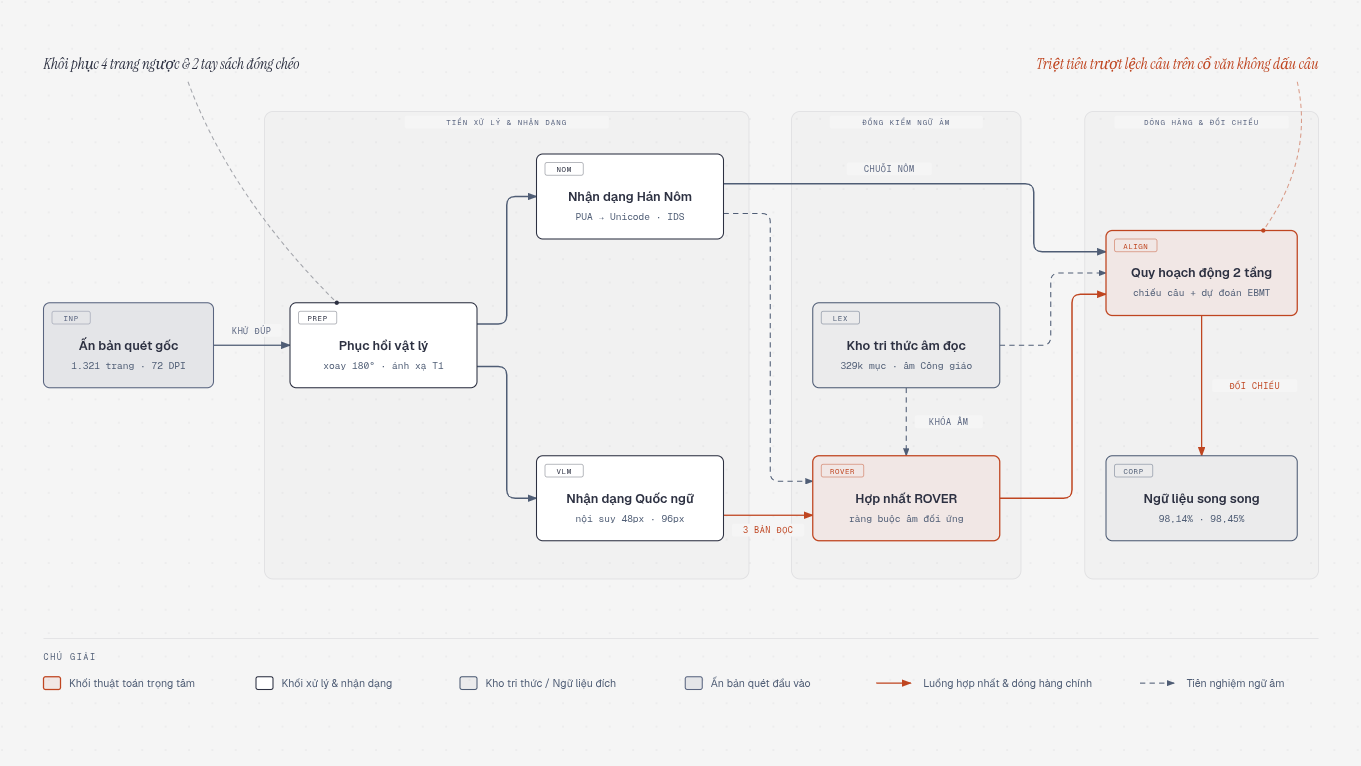
\includegraphics[width=\linewidth]{images/fig1-arch.png}
    \caption{Kiến trúc tổng thể quy trình xây dựng ngữ liệu song song Hán Nôm -- Quốc ngữ từ ấn bản lịch sử}
    \label{fig:arch}
\end{figure}

\subsection{Phân tích mật độ điểm ảnh gốc và trích xuất bảo toàn thông tin}

Trong nhiều quy trình số hóa tài liệu, ảnh trang sách thường được kết xuất ở độ phân giải $300\text{ DPI}$ với kỳ vọng cải thiện độ nét cho mô hình nhận dạng. Tuy nhiên, khi kiểm tra trực tiếp luồng ảnh nhúng bên trong tệp quét gốc của hai tập sách, nhóm ghi nhận các trang ảnh thực chất đã được số hóa ở mật độ xấp xỉ $72\text{ DPI}$, tương ứng với kích thước khoảng $800 \times 1135$ đến $1067 \times 1513$ điểm ảnh. Xét theo nguyên lý lấy mẫu tín hiệu, việc phóng toàn trang lên $300\text{ DPI}$ chỉ tạo ra nội suy phóng đại gấp khoảng $4{,}17$ lần mỗi chiều, làm tăng dung lượng lưu trữ khoảng $5{,}5$ lần mà không bổ sung thêm chi tiết tần số cao thực sự cho bộ nhận dạng toàn trang.

Từ quan sát đó, nhóm quyết định trích xuất ảnh trang ở đúng độ phân giải gốc $72\text{ DPI}$ nhằm giữ nguyên phân bố mức xám ban đầu cho luồng nhận dạng Hán Nôm và tiết kiệm dung lượng lưu trữ. Ở nhánh Quốc ngữ, phép nội suy phóng đại chỉ được áp dụng có chọn lọc ở mức từng dòng chữ đã cắt rời bằng bộ lọc Lanczos bậc cao khi đưa vào mô hình thị giác, nhằm đáp ứng kích thước lưới vi mảnh của bộ mã hóa ảnh mà không làm phình kích thước tập ảnh gốc.

\subsection{Mô hình hóa ánh xạ trang tuyến tính từng đoạn}

Sau khi loại bỏ hai trang quét đúp ở Tập 2 và tách riêng các trang không thuộc chính văn (bìa, lời tựa, mục lục, chú thích và trang trắng), gọi $\mathcal{I}_{\text{vi}}$ và $\mathcal{I}_{\text{ch}}$ lần lượt là tập chỉ số trang chính văn Quốc ngữ và Hán Nôm. Do Tập 1 có trang trắng xen giữa, hai cặp tay sách bị hoán vị và hai trang Quốc ngữ bị quét thiếu, quan hệ ghép trang không thể biểu diễn bằng một công thức tuyến tính đơn lẻ cho cả hai tập, mà được mô hình hóa dưới dạng hàm tuyến tính từng đoạn theo thứ tự đọc xuôi của vế Quốc ngữ và thứ tự đọc ngược của vế Hán Nôm.

Đối với Tập 2 ($683$ trang hiệu lực sau khi loại hai trang trùng thứ $27$ và $28$), cấu trúc đối xứng được duy trì liên tục trên toàn bộ $331$ cặp trang chính văn theo biểu thức:
\begin{equation}
    f_{\text{Tập 2}}(p_{\text{vi}}) = 681 - p_{\text{vi}}, \quad \forall p_{\text{vi}} \in [7, 337].
\end{equation}
Trái lại, trên Tập 1 ($636$ trang), ánh xạ $f_{\text{Tập 1}}: \mathcal{I}_{\text{vi}} \to \mathcal{I}_{\text{ch}}$ cần được phân rã thành bảy miền liên tiếp nhằm phản ánh chính xác hai cặp tay sách đóng chéo và bước nhảy pha $\Delta = -2$ sau hai trang Hán Nôm khuyết vế Quốc ngữ ($p_{\text{ch}} \in \{359, 358\}$):
\begin{equation}
    f_{\text{Tập 1}}(p_{\text{vi}}) =
    \begin{cases}
        635 - p_{\text{vi}}, & p_{\text{vi}} \in [11, 17] \cup [19, 42] \cup [45, 52] \cup [55, 275] \\
        625 - p_{\text{vi}}, & p_{\text{vi}} \in [43, 44] \quad \text{(hoán vị tay sách thứ nhất: } 582, 581\text{)} \\
        645 - p_{\text{vi}}, & p_{\text{vi}} \in [53, 54] \quad \text{(hoán vị tay sách thứ hai: } 592, 591\text{)} \\
        633 - p_{\text{vi}}, & p_{\text{vi}} \in [276, 314] \quad \text{(dịch pha } \Delta = -2 \text{ sau } 2 \text{ trang khuyết).}
    \end{cases}
\end{equation}
Để tránh sai sót thủ công khi khai báo các miền trang, quá trình phân hoạch luôn đi kèm bước kiểm tra tự động ba điều kiện đóng: các nhóm trang không giao nhau và phủ kín khoảng $[1, N_{\text{trang}}]$, tập ảnh xuất hiện ở hai vế của bảng ghép trang trùng khớp với tập trang chính văn, và toàn bộ ảnh sau khi xoay phục hồi $180^\circ$ bốn trang quét ngược đều giữ chiều đứng ($W < H$).

\subsection{Tách vùng chính văn bằng hình thái học và thống kê bền vững}

Đặc điểm chung của các trang in khắc đầu thế kỷ XX là sự hiện diện của khung viền hoa văn kép bao quanh vùng chữ, dòng số trang in ở lề trên trang Quốc ngữ (có dạng \code{- 53 - ( 584 )}) và tên sách kèm số tờ bằng chữ Hán ở mép gáy ngoài khung của trang Nôm. Nếu giữ lại các thành phần rìa này trong chuỗi văn bản đầu vào, chúng sẽ tạo ra sự chênh lệch không có đối ứng giữa hai vế và làm giảm trực tiếp độ tương đồng khi dóng hàng.

Nhằm lọc sạch các nhiễu rìa mà không vô tình xóa mất cột kết đoạn ngắn ở cuối mục, hệ thống áp dụng bộ lọc hình học hai nhánh thích ứng theo kích thước từng trang. Trên trang Hán Nôm, các cột văn bản chuẩn bên trong khung được xác định từ những vùng nhận dạng có độ dài tối thiểu $8$ ký tự, từ đó ước lượng biên bao $[x_{\min}, x_{\max}] \times [y_{\min}, y_{\max}]$ cùng trung vị độ rộng cột $\tilde{w} = \operatorname{median}_k(w_k)$. Một khung hộp có tâm $(x_c, y_c)$ và kích thước $(w, h)$ sẽ bị loại nếu nằm ngoài lề ngang với dung sai bất đối xứng về bên trái ($x_c < x_{\min} - 1{,}45\tilde{w}$ nhằm giữ lại cột ngắn kết thúc đoạn theo chiều đọc phải sang trái, hoặc $x_c > x_{\max} + 0{,}8\tilde{w}$ ở lề phải), vượt quá biên dọc $y_c \notin [y_{\min} - 0{,}5\tilde{w},\; y_{\max} + 0{,}5\tilde{w}]$, quá mảnh như đoạn đường kẻ khung bị nhận nhầm ($w < 0{,}48\tilde{w}$), hoặc là nhiễu đơn tự kéo dài bất thường ($|\text{chuỗi}| = 1$ và $h / w > 3{,}5$). Tương tự, trên trang Quốc ngữ, đỉnh vùng thân trang $y_{\text{body}}$ được ước lượng từ cực tiểu tung độ của các dòng văn bản thông thường (có ít nhất $15$ ký tự), cho phép tách bỏ có chọn lọc các dòng tiêu đề số trang nằm tách biệt phía trên trước khi ghép dòng.

\begin{softbox}
\textbf{Nhận xét kỹ thuật:} Việc sử dụng trung vị độ rộng cột $\tilde{w}$ thay cho giá trị trung bình giúp các ngưỡng lọc ít bị ảnh hưởng bởi những khung hộp ngoại lai (chẳng hạn hai cột chập dính vào nhau hoặc vết chấm mực ở mép giấy), đồng thời giữ tính ổn định khi tỷ lệ kích thước ảnh thay đổi giữa các trang quét.
\end{softbox}

\section{Nhận Dạng Quang Học Đa Mô Hình và Chuẩn Hóa Tự Hình -- Chính Tả}

\subsection{Giải mã vùng sử dụng riêng (PUA) và hiệu chỉnh tự hình bằng cấu trúc biểu ý (IDS)}

Trong thực tế nhận dạng văn bản Hán Nôm khắc in, một phần đáng kể sai số dóng hàng không bắt nguồn từ thuật toán so khớp mà phát sinh ngay từ sự lệch chuẩn mã ký tự và hiện tượng nhầm lẫn giữa các tự hình gần nét. Trước hết, bộ nhận dạng chuyên dụng cho chữ Nôm thường xuất ra các điểm mã nằm trong vùng sử dụng riêng (\code{U+F0000}--\code{U+FFFFD}) đối với những chữ Nôm chưa có trong các bảng mã cũ. Vì các mã PUA này không khớp trực tiếp với các từ điển chuẩn hóa theo Unicode hiện đại (CJK Extension G, H, I), hệ thống sẽ đánh dấu chúng là ký tự ngoài từ điển nếu không quy đổi trước. Thông qua việc đối chiếu mã nguồn chữ Việt trong cơ sở dữ liệu Unihan \cite{unihan2025} kết hợp phân tích chuỗi mô tả cấu trúc biểu ý (IDS) \cite{morioka2008ids} trực tiếp trên ảnh khắc in gốc, toàn bộ $25$ loại mã PUA xuất hiện trong hai tập sách đã được rà soát và phân định rõ ràng. Trong số này, $24$ loại tự hình đã được ánh xạ về đúng điểm mã Unicode chính thức, chẳng hạn \nom{𱥺} (\code{U+3197A}, \textit{một}), \nom{𱏺} (\code{U+313FA}, \textit{sách}), \nom{𱺵} (\code{U+31EB5}, \textit{là}), \nom{𲈳} (\code{U+32233}) và \nom{𲈫} (\code{U+3222B}, \textit{cửa}), \nom{𩈘} (\code{U+29218}, cấu trúc \ids{⿰}\nom{末面}, \textit{mặt}), \nom{𫢩} (\code{U+2B8A9}, \ids{⿰}\nom{尼今}, \textit{nay}) hay \nom{𣌋} (\code{U+2330B}, \ids{⿱}\nom{日歛}, \textit{sớm}). Nhờ bước quy đổi này, Tập 1 không còn ký tự đại diện ngoài chuẩn nào ($0$ ký tự \nom{〓}), còn trên Tập 2 chỉ duy nhất $1$ loại tự hình (ứng với mã nhận dạng thô \code{U+F0815}, xuất hiện một lần tại trang $387$, câu thứ $7$) mang cấu trúc biểu ý \ids{⿱}\nom{𥫗頓} (bộ trúc \nom{𥫗} phía trên, chữ đốn \nom{頓} biểu âm phía dưới, đọc là \textit{lớn}) thực sự chưa có trong chuẩn Unicode hiện hành; trường hợp này được biểu diễn bằng ký hiệu \nom{〓} (\code{U+3013}) và lưu hồ sơ tọa độ chi tiết ở cả mức cột, mức ô chữ đơn và mức câu.

Song song với khâu giải mã PUA, quá trình khảo sát ảnh bản in cho thấy khi nét khắc bị mòn hoặc mực in nhòe cục bộ, bộ nhận dạng thị giác có xu hướng đưa một số chữ Nôm tần suất cao về các chữ Hán phổ thông có bố cục bộ thủ gần giống. Dựa trên đối chiếu trực tiếp nét khắc với cấu trúc IDS, nhóm đã tổng hợp bảng quy đổi cho $19$ cặp tự hình bị nhận nhầm mang tính hệ thống xuyên suốt cả hai tập sách; Bảng~\ref{tab:glyph_fix} minh họa một số quy luật tiêu biểu cùng nguyên nhân thị giác tương ứng.

\begin{table}[H]
    \centering
    \footnotesize
    \renewcommand{\arraystretch}{1.22}
    \begin{tabularx}{\textwidth}{c c c c X}
        \toprule
        \textbf{Nhận nhầm} & \textbf{Tự hình đúng} & \textbf{Cấu trúc IDS} & \textbf{Âm đọc} & \textbf{Cơ chế gây nhầm lẫn thị giác trên bản in cổ} \\
        \midrule
        \nom{𠯇} / \nom{吔} & \nom{吧} (\texttt{U+5427}) & \ids{⿰}\nom{口巴} & \textit{và} & Nét sổ giữa của bộ \nom{巴} bị đứt hoặc dính vào nét móc, nhìn giống \nom{巳} hoặc \nom{也} \\
        \nom{髀} & \nom{𪡔} (\texttt{U+2A854}) & \ids{⿰}\nom{口}\ids{⿱}\nom{罒廾} & \textit{ra} & Bộ \nom{口} và \ids{⿱}\nom{罒廾} xếp sát nhau bị nhận nhầm thành bộ \nom{骨} và \nom{卑} \\
        \nom{樓} & \nom{𢖕} (\texttt{U+22595}) & \ids{⿰}\nom{後娄} & \textit{sau} & Bộ \nom{彳} (\nom{後}) nét mảnh bị nhầm sang bộ \nom{木} của chữ Hán phổ thông \nom{樓} \\
        \nom{𠺌} & \nom{魂} (\texttt{U+9B42}) & \ids{⿰}\nom{云鬼} & \textit{hồn} & Phần \nom{云} in nhỏ bên trái bị nhầm thành bộ \nom{口} \\
        \nom{僃} & \nom{𡞕} (\texttt{U+21795}) & \ids{⿰}\nom{女备} & \textit{vợ} & Bộ \nom{女} hẹp ngang bị nhầm thành bộ nhân đứng \nom{亻} \\
        \nom{肄} & \nom{𤈠} (\texttt{U+24220}) & \ids{⿰}\nom{火聿} & \textit{sốt} & Bộ \nom{火} ở vế trái bị mờ nét chấm, nhầm sang vế trái của \nom{肄} \\
        \nom{聰} / \nom{課} & \nom{嚕} / \nom{𠵩} & \ids{⿰}\nom{口魯} / \ids{⿰}\nom{口果} & \textit{rủa} / \textit{quở} & Bộ \nom{口} của chữ Nôm biểu ý lời nói bị nhầm sang bộ \nom{耳} và \nom{言} \\
        \nom{海} / \nom{𬇚} & \nom{泑} (\texttt{U+6CD1}) & \ids{⿰}\nom{氵幼} & \textit{ao} & Vế biểu âm \nom{幼} nhòe mực bị kéo về chữ Hán tần suất cao \nom{海} \\
        \nom{配} / \nom{盆} & \nom{醜} / \nom{益} & \ids{⿰}\nom{酉鬼} / \ids{⿱}\ids{⿰}\nom{丷一}\ids{⿱}\nom{八皿} & \textit{xấu} / \textit{ích} & Khuyết nét bên phải (\nom{鬼}) hoặc nhòe phần đầu chữ \nom{益} \\
        \bottomrule
    \end{tabularx}
    \caption{Một số quy luật nhầm lẫn tự hình Hán Nôm mang tính hệ thống và phân giải theo IDS}
    \label{tab:glyph_fix}
\end{table}

\subsection{Nhận dạng Quốc ngữ bằng mô hình ngôn ngữ -- thị giác trên khung dòng nội suy}

Các thử nghiệm bước đầu trên bản in Quốc ngữ đầu thế kỷ XX cho thấy hai họ mô hình nhận dạng có điểm mạnh và điểm yếu bổ trợ cho nhau. Một mặt, bộ nhận dạng dòng truyền thống dựa trên mạng hồi quy LSTM như Tesseract định vị khung tọa độ của từng dòng chữ khá ổn định, nhưng khi đọc nội dung lại thường xuyên sai dấu thanh điệu và nhầm lẫn các cặp ký tự gần hình như \textit{d/đ}, \textit{i/l}, \textit{ch/cb}, \textit{th/tb} hoặc lặp nguyên âm mang dấu (ví dụ \textit{tộôi}). Mặt khác, nếu đưa nguyên cả trang ảnh vào một mô hình ngôn ngữ -- thị giác đa phương thức (VLM) \cite{bai2025qwenvl}, mô hình có khả năng đọc dấu tiếng Việt tốt hơn nhưng lại dễ bỏ sót dòng, chập hai dòng liền kề hoặc tự ý diễn giải từ cổ theo chính tả hiện đại.

Để tận dụng thế mạnh của cả hai hướng tiếp cận, luồng nhận dạng Quốc ngữ được tách thành hai pha gắn chặt theo không gian dòng. Ở pha đầu tiên, trang ảnh được phân hoạch thành danh sách có thứ tự các hộp bốn điểm bao sát từng dòng ngang $B_1, B_2, \dots, B_L$, ưu tiên sử dụng khung dòng từ bộ phân tích bố cục truyền thống (và có thể thay bằng phân tích thành phần liên thông hình thái học khi vận hành độc lập). Sang pha thứ hai, từng vùng dòng $B_\ell$ được cắt rời kèm phần đệm biên $4\text{ px}$; nếu chiều cao dòng nhỏ hơn ngưỡng $h_{\min}$ ($48\text{ px}$ ở lượt chính), ảnh dòng sẽ được phóng đại đẳng hướng bằng bộ lọc Lanczos bậc 4 ($\operatorname{sinc}$ cửa sổ $8 \times 8$) trước khi đưa vào mô hình Qwen3-VL-8B-Instruct ở chế độ suy luận tất định ($T = 0$). So với phép nội suy song tuyến tính thông thường, bộ lọc Lanczos giữ độ sắc nét tốt hơn ở nét gạch ngang chữ \textit{đ} cũng như khoảng hở giữa dấu mũ và dấu thanh điệu.

Bên cạnh đó, đối với giả thuyết sinh ra từ bộ nhận dạng truyền thống, nhóm áp dụng thêm một bộ lọc hậu xử lý chính tả có điều kiện nhằm bảo toàn từ cổ. Gọi $\mathcal{V}_{\text{vi}}$ là tập hợp các âm tiết đơn tiếng Việt hợp lệ trích xuất từ kho từ điển; một từ $w$ chỉ được đưa vào diện xét sửa khi $w \notin \mathcal{V}_{\text{vi}}$, thông qua tập ứng viên biến đổi tối tiểu $\mathcal{C}(w)$ đặc trưng cho lỗi quang học (khử nguyên âm đúp cùng gốc không dấu, rút gọn lỗi chập \textit{dđ} thành \textit{đ}, khôi phục \textit{b} thành \textit{h} sau các phụ âm đầu \textit{c, t, k, p, g, n}), và ứng viên $w' \in \mathcal{C}(w)$ chỉ được chấp nhận nếu $w' \in \mathcal{V}_{\text{vi}}$. Ràng buộc điều kiện $w \notin \mathcal{V}_{\text{vi}}$ giúp các hình thái chính tả cổ vốn có mặt trong từ điển lịch sử như \textit{chưng, lọn, lở, hằng, phô} cũng như danh từ riêng có gạch nối (\textit{Phê-rô, Giê-su}) không bị sửa nhầm sang từ hiện đại.

\subsection{Hợp nhất giả thuyết ROVER có ràng buộc ngữ âm liên ngôn ngữ}

Ngay cả khi sử dụng mô hình thị giác 8 tỷ tham số trên ảnh dòng đã nội suy, các trang giấy ố vàng nặng hoặc in nhạt ở nét phụ vẫn phát sinh một tỷ lệ nhỏ lỗi bỏ sót nét ngang chữ \textit{đ} (chẳng hạn đọc \textit{đàng} thành \textit{dàng}, \textit{Đấng} thành \textit{Dấng}) hoặc nhầm giữa các nguyên âm có dấu phụ gần nhau (\textit{ư/u}, \textit{ơ/ô}, \textit{ă/â}). Trong nhận dạng tiếng nói và văn bản, kỹ thuật ROVER (Recognizer Output Voting Error Reduction) \cite{fiscus1997rover} thường kết hợp nhiều giả thuyết bằng bỏ phiếu đa số; tuy nhiên, khi số lượng mô hình nhỏ và các mô hình đều có xu hướng nghiêng về từ tiếng Việt hiện đại phổ biến hơn, bỏ phiếu không ràng buộc khó phân biệt được đâu là cách đọc đúng với bản khắc cổ.

Từ nhận xét trên, nhóm áp dụng cơ chế \textbf{ROVER có ràng buộc ngữ âm liên ngôn ngữ}, sử dụng trực tiếp chuỗi chữ Hán Nôm của trang đối ứng làm tín hiệu chọn lọc giữa ba luồng giả thuyết độc lập trên cùng một hộp dòng $B_\ell$: giả thuyết chính $H^{(1)}_\ell$ từ Qwen3-VL-8B ở độ cao chuẩn hóa $48\text{ px}$, giả thuyết đối chứng $H^{(2)}_\ell$ từ bộ nhận dạng truyền thống sau hậu xử lý, và giả thuyết độ phân giải cao $H^{(3)}_\ell$ từ Qwen3-VL-8B ở chiều cao $96\text{ px}$ với chỉ dẫn chú trọng các cặp nét vi mô (\textit{d/đ}, \textit{ă/â/ê/ô/ơ/ư}). Với mỗi trang Quốc ngữ thuộc cặp ánh xạ thứ $i$, hệ thống xét cửa sổ ba cặp trang liên tiếp $\mathcal{W}_i = \{i-1, i, i+1\}$ để bao quát cả các câu vắt qua ranh giới chuyển trang. Gọi $\mathcal{C}(\mathcal{W}_i)$ là tập mọi tự hình Hán Nôm xuất hiện trong cửa sổ $\mathcal{W}_i$ và $\mathcal{R}_0(c)$ là tập khóa âm tiết (chuẩn hóa NFC, viết thường, lược bỏ năm dấu thanh nhưng giữ nguyên phân biệt nguyên âm có dấu phụ và phụ âm \textit{d/đ}) của tự hình $c$ trong kho từ điển tổng hợp; không gian khóa ngữ âm khả dĩ của vùng trang được xác định bởi:
\begin{equation}
    \mathcal{K}_i = \bigcup_{c \in \mathcal{C}(\mathcal{W}_i)} \mathcal{R}_0(c).
\end{equation}

Tiếp theo, định nghĩa phép chiếu khung chữ cái cơ sở $\beta(w)$ chuyển mỗi từ tiếng Việt về chuỗi chữ cái Latinh không dấu (ví dụ $\beta(\text{``đàng''}) = \beta(\text{``dàng''}) = \text{``dang''}$ và $\beta(\text{``chưng''}) = \beta(\text{``chúng''}) = \text{``chung''}$). Khi so khớp giả thuyết chính $H^{(1)}_\ell = (w_1, \dots, w_p)$ với từng giả thuyết phụ $H^{(m)}_\ell = (u_1, \dots, u_q)$ ($m \in \{2, 3\}$), hệ thống tìm các đoạn khớp dài nhất trên hai dãy khung cơ sở $(\beta(w_r))$ và $(\beta(u_s))$. Tại mỗi cặp từ đối ứng $(w_r, u_s)$ có cùng khung cơ sở $\beta(w_r) = \beta(u_s)$ nhưng khác nhau ở dấu phụ hoặc nét \textit{d/đ}, từ $u_s$ (giữ nguyên quy cách viết hoa của $w_r$) chỉ được chọn thay cho $w_r$ khi thỏa mãn đồng thời điều kiện bất đối xứng:
\begin{equation}
    \phi(w_r) \notin \mathcal{K}_i \quad \land \quad \phi(u_s) \in \mathcal{K}_i,
\end{equation}
trong đó $\phi(\cdot)$ là hàm trích khóa âm tiết giữ nguyên dấu phụ chữ cái.

\begin{softbox}
\textbf{Đặc tính an toàn của luật chọn lọc:} Do chỉ lựa chọn giữa các từ thực sự do các bộ nhận dạng đọc ra trên cùng hộp dòng, cơ chế ROVER liên ngôn ngữ tránh được việc tự sinh từ ngoài ảnh gốc. Đồng thời, điều kiện bất đối xứng đảm bảo giả thuyết chính chỉ bị thay thế khi khóa âm của nó không khớp với bất kỳ tự hình Nôm nào trong cửa sổ ba trang đối ứng, trong khi giả thuyết phụ lại khớp trực tiếp với một tự hình hiện diện trên trang.
\end{softbox}

\section{Tri Thức Từ Vựng Học, Phân Đoạn Câu và Dóng Hàng Quy Hoạch Động Hai Tầng}

\subsection{Hợp nhất không gian từ điển đa nguồn và hệ âm đọc Nôm Công giáo}

Hiệu quả của các bước dóng hàng ngữ âm phụ thuộc trực tiếp vào độ phủ của ánh xạ giữa tự hình Hán Nôm và tập âm đọc hợp lệ $\mathcal{L}(c)$. Để giảm thiểu số trường hợp báo lệch do thiếu mục từ, hệ thống tổng hợp tri thức từ bảy nguồn từ điển ngữ văn và từ nguyên quy mô lớn, bao gồm \textit{Bảng chữ Hán Nôm chuẩn} ($8.855$ mục), \textit{Bảng Tra Chữ Nôm} ($13.443$ mục), \textit{Digitizing Vietnam} ($53.959$ mục), \textit{Đại Nam Quấc Âm Tự Vị} ấn bản năm $1895$ \cite{huinhtinh1895} ($70.364$ mục), \textit{Từ điển Hán Nôm HVDIC} ($50.332$ mục), cơ sở dữ liệu \textit{Unihan} \cite{unihan2025} ($132.698$ mục) cùng bảng quan hệ chữ dị thể \textit{CJKVI}. Sau khi chuẩn hóa về dạng dựng sẵn NFC, kho từ vựng hợp nhất đạt tổng cộng $329.651$ mục âm đọc, trong đó có $198.438$ mục âm Hán-Việt, Nôm và Quốc ngữ phủ trên $90.834$ tự hình đơn nhất, đi kèm $122.350$ liên kết dị thể hai chiều $V(c)$ giúp nhận diện các biến thể khắc chữ tương đương nhau về ngữ âm.

Mặc dù kho từ điển chung có độ phủ rộng, khảo sát trực tiếp trên hai tập sách cho thấy văn hiến Công giáo Việt Nam thế kỷ XVII--XX sử dụng một lớp từ vựng ký âm riêng lặp lại nhiều lần mà các từ điển thế tục không ghi nhận đầy đủ. Lớp từ vựng này gồm hai nhóm chính: nhóm danh từ riêng thần học đa âm tiết phiên âm từ tiếng Latinh hoặc Bồ Đào Nha như \nom{支秋} (\textit{Giê-su}, với \nom{秋} ghi âm \textit{su}), \nom{衣計移加} (\textit{I-ghe-rê-gia}, phiên âm từ \textit{Ecclesia} với \nom{計} đọc \textit{ghe} và \nom{移} đọc \textit{rê}), \nom{樞姚} (\textit{Giu-dêu}) hay \nom{樞蜂} (\textit{Giu-ong}); và nhóm chữ giả tá hay chuyển âm cổ trong ngữ cảnh giáo lý như \nom{最思} (\textit{tối tăm}, dùng \nom{思} đọc \textit{tăm}), \nom{諫讓} (\textit{khiêm nhường}, \nom{諫} đọc \textit{khiêm}), \nom{識傳} (\textit{Sấm Truyền}, \nom{識} đọc \textit{sấm}), \nom{偃㑏} (\textit{gìn giữ}, \nom{偃} đọc \textit{gìn}), \nom{𢗼憫} (\textit{lo lắng}, \nom{憫} đọc \textit{lắng}) và \nom{嚉靈魂} (\textit{rỗi linh hồn}, trong đó \nom{嚉} mang thêm âm \textit{rỗi} bên cạnh âm \textit{dối} thông thường). Việc bổ sung có chọn lọc lớp âm đọc chuyên biệt này vào không gian tra cứu giúp thuật toán dóng hàng phản ánh đúng tập quán ký âm của tác phẩm thay vì đánh dấu nhầm các thuật ngữ tôn giáo là lỗi nhận dạng.

\subsection{Khôi phục từ vắt dòng, nối câu xuyên trang và phân đoạn câu theo ngữ cảnh}

Trước khi thực hiện dóng hàng, các chuỗi văn bản rời rạc theo dòng và theo trang cần được tái cấu trúc thành những đơn vị câu hoàn chỉnh. Trên ấn bản Quốc ngữ đầu thế kỷ XX, trở ngại đầu tiên nằm ở dấu gạch nối cuối dòng vì nó vừa có thể là dấu nối nội tại của danh từ riêng phiên âm (như \textit{Giê-su}, \textit{Phi-ri-tô}), vừa có thể chỉ là ký hiệu ngắt dòng cơ học khi hết lề phải. Để phân giải sự nhập nhằng này, hệ thống xét đặc trưng viết hoa của hai mảnh $p_1\text{-}p_2$ qua điểm ngắt dòng: dạng nối liền $p_1\text{-}p_2$ được giữ lại khi cả hai mảnh đều viết hoa chữ cái đầu hoặc thuộc danh mục từ ghép cố định, còn các trường hợp từ thông thường được khôi phục thành hai âm tiết cách nhau bởi khoảng trắng.

Tiếp theo, do nhiều câu văn bắt đầu ở cuối trang $t$ và kéo dài sang đầu trang $t+1$, việc tách câu độc lập trên từng trang sẽ cắt đôi những câu vắt trang thành các mảnh thiếu đối ứng. Nhằm tránh hiện tượng này, hệ thống kiểm tra ký tự hữu ích cuối cùng trên vế Quốc ngữ của mỗi cặp trang (bỏ qua dấu đóng ngoặc hoặc dấu ngoặc kép đi kèm); nếu chưa xuất hiện dấu kết câu (\code{. ? ! ; : \ldots}), cặp trang hiện tại được gộp liên thông với cặp trang kế tiếp thành một cụm trang thống nhất trước khi phân đoạn, đồng thời lưu lại khoảng chỉ số ký tự của từng trang gốc để gán đúng định danh câu về trang chứa ký tự mở đầu. Trên chuỗi Quốc ngữ đã nối cụm trang, bộ phân đoạn ranh giới câu hoạt động theo hướng xét ngữ cảnh lấy cảm hứng từ mô hình Punkt \cite{kiss2006punkt}: thay vì tách cơ học tại mọi dấu chấm, thuật toán kiểm tra cặp từ liền kề $(w_i, w_{i+1})$ để không ngắt câu sau các chữ viết tắt đa chấm (\textit{v.v.}, \textit{đ.c.}) và viết tắt tôn giáo -- học thuật (\textit{Lm.}, \textit{Th.}, \textit{St.}, \textit{Đc.}, \textit{tr.}), không ngắt tại trích dẫn Kinh Thánh có ký hiệu sách (\textit{Mt, Mc, Lc, Ga, Rm, Cr, Tv,\ldots}) đi kèm số chương hoặc số câu, và không ngắt sau chữ số La Mã chỉ thứ tự mục khi từ kế tiếp $w_{i+1}$ bắt đầu bằng chữ cái viết thường hoặc không mang dấu hiệu mở câu mới.

\subsection{Quy hoạch động hai tầng}

Thách thức lớn nhất khi dóng hàng giữa văn bản Hán Nôm và bản phiên âm Quốc ngữ xuất phát từ sự chênh lệch về độ tin cậy của dấu ngắt câu ở hai hệ chữ viết. Trong khi bản Quốc ngữ có hệ thống dấu câu và quy tắc viết hoa đầu câu tương đối rõ ràng, bản Hán Nôm lại có nhiều đoạn kéo dài không chấm câu hoặc dùng dấu khuyên tròn \nom{。} lệch vị trí so với dấu chấm câu Quốc ngữ. Nếu tách câu độc lập trên cả hai vế rồi mới ghép cặp ở mức câu, chỉ một vài chỗ tách sai ở đầu trang cũng có thể kéo theo sai lệch cho các câu kế tiếp. Để khắc phục hạn chế này, quy trình dóng hàng được thiết kế theo mô hình \textbf{quy hoạch động phân cấp hai tầng} kết nối trực tiếp với kết quả từ bước hợp nhất ROVER như trình bày ở Hình~\ref{fig:rover_dp}.

\begin{figure}[H]
    \centering
    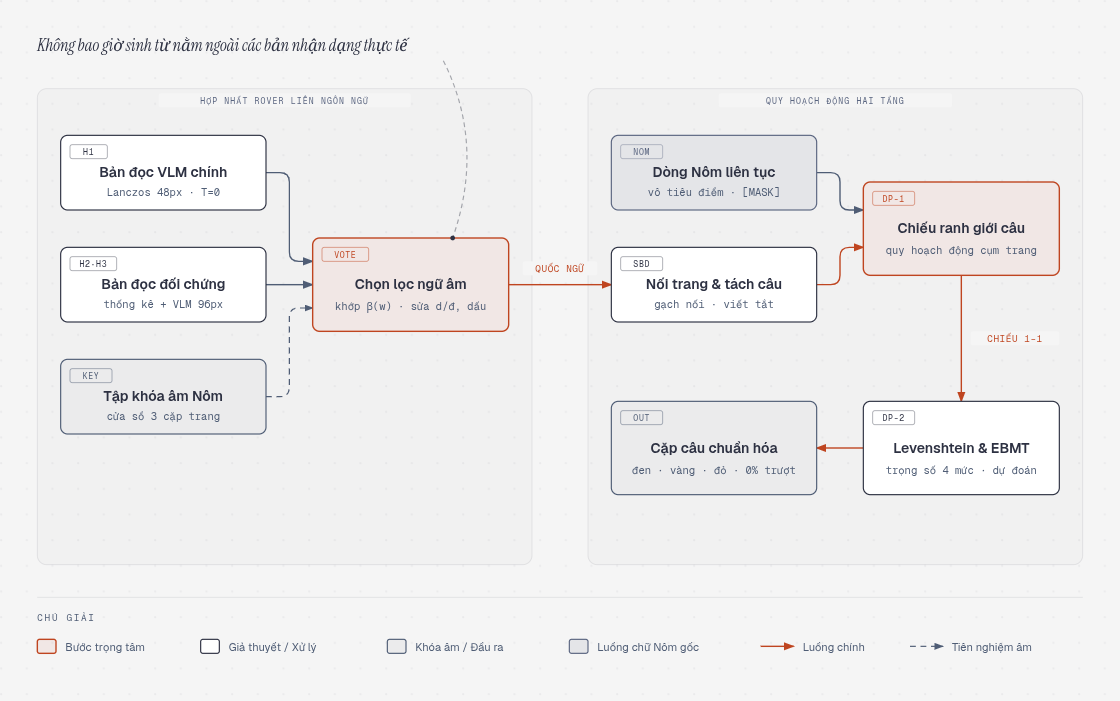
\includegraphics[width=0.95\linewidth]{images/fig2-rover-dp.png}
    \caption{Cơ chế hợp nhất ROVER liên ngôn ngữ kết nối với quy hoạch động phân cấp hai tầng}
    \label{fig:rover_dp}
\end{figure}

\subsubsection{Tầng 1: Chiếu ranh giới câu cấp độ cụm trang}

Trên mỗi cụm trang đã nối xuyên trang, gọi $C = (c_1, c_2, \dots, c_N)$ là dãy toàn bộ phần tử Hán Nôm (giữ nguyên dấu câu tại vị trí gốc và xem ký hiệu khuyết chữ \code{[MASK]} là một phần tử nguyên tử không chia tách) và gọi $S^{(1)}, S^{(2)}, \dots, S^{(K)}$ là $K$ câu Quốc ngữ đã tách theo ngữ cảnh, tạo thành dãy gồm $M$ âm tiết $S = (s_1, s_2, \dots, s_M)$ với các mốc ranh giới câu tích lũy $0 = \tau_0 < \tau_1 < \dots < \tau_K = M$. Thay vì tìm ranh giới câu trên vế Hán Nôm bằng dấu câu, tầng thứ nhất căn chỉnh trực tiếp chuỗi $C$ với chuỗi $S$ qua ma trận quy hoạch động $D \in \mathbb{R}^{(N+1) \times (M+1)}$ được xác định bởi điều kiện biên $D(0, 0) = 0$, $D(i, 0) = i$, $D(0, j) = j$ cùng hệ thức truy hồi:
\begin{equation}
    D(i, j) = \min
    \begin{cases}
        D(i-1, j-1) + \delta_{\text{lex}}(c_i, s_j) & \text{(khớp hoặc thay thế)} \\
        D(i-1, j) + 1 & \text{(xóa phần tử Nôm, bao gồm dấu câu Nôm)} \\
        D(i, j-1) + 1 & \text{(chèn âm tiết Quốc ngữ),}
    \end{cases}
\end{equation}
trong đó chi phí ngữ âm $\delta_{\text{lex}}(c_i, s_j)$ bằng $0$ nếu $s_j$ thuộc tập âm đọc trực tiếp $\mathcal{L}(c_i)$ hoặc tập âm đọc qua quan hệ dị thể $\bigcup_{v \in V(c_i)} \mathcal{L}(v)$, và bằng $1$ trong trường hợp còn lại.

Khi truy vết đường đi có tổng chi phí nhỏ nhất từ $(N, M)$ ngược về $(0, 0)$, các bước đi chéo xác định một ánh xạ đơn điệu không giảm $\mu: \operatorname{Dom}(\mu) \subseteq \{1,\dots,M\} \to \{1,\dots,N\}$. Với mỗi câu Quốc ngữ thứ $k$ nằm trên dải âm tiết $(\tau_{k-1}, \tau_k]$, chỉ số cắt kết thúc tương ứng trên dòng Hán Nôm $e_k$ được xác định tuần tự từ $e_0 = 0$ như sau:
\begin{equation}
    e_k =
    \begin{cases}
        N, & \text{nếu } k = K \\
        \max\Big(e_{k-1},\; \max\big\{\mu(j) \;\big|\; j \in (\tau_{k-1}, \tau_k] \cap \operatorname{Dom}(\mu)\big\}\Big), & \text{nếu tập ánh xạ khác rỗng} \\
        e_{k-1}, & \text{ngược lại.}
    \end{cases}
\end{equation}
Đoạn con liên tục $C[e_{k-1}+1 : e_k]$ chính là vế Hán Nôm tương ứng với câu Quốc ngữ thứ $k$, và mọi phân đoạn biên bị rỗng một vế (nếu phát sinh) sẽ được gộp vào câu liền kề. Nhờ cấu trúc phân hoạch nối tiếp này, tổng hợp tất cả các lát cắt câu luôn khớp từng ký tự với dòng Hán Nôm gốc trên cụm trang ($\bigoplus_{k=1}^K C^{(k)} \equiv C$), không làm rơi ký tự hay xé lẻ ký hiệu \code{[MASK]}. Quan trọng hơn, vì mỗi điểm cắt câu đều bám vào vị trí khớp ngữ âm thực trên toàn cụm trang thay vì dựa vào dấu \nom{。}, nhiễu cục bộ ở một câu không làm trượt ranh giới của những câu phía sau, giúp giữ tỷ lệ hàng không so sánh ở mức $0{,}00\%$ trên cả hai tập sách.

\subsubsection{Tầng 2: Đối chiếu chỉnh sửa Levenshtein có trọng số ngữ âm và phân lớp sai khác}

Sau khi có từng cặp câu 1--1 $(C^{(k)}, S^{(k)})$ ở dạng chuẩn hóa NFC, tầng thứ hai đối chiếu chi tiết từng tự hình Nôm với từng âm tiết Quốc ngữ. Trước hết, nếu hai vế có cùng số lượng ký hiệu khuyết chữ \code{[MASK]}, cặp câu được tách theo các điểm neo này để dóng hàng độc lập trên từng đoạn con, đảm bảo ký hiệu \code{[MASK]} luôn ở trạng thái trung lập và không bị tính là lỗi. Trên mỗi phân đoạn gồm dãy tự hình Nôm $(x_1, \dots, x_p)$ và dãy âm tiết hoặc số Quốc ngữ $(y_1, \dots, y_q)$, thuật toán khoảng cách chỉnh sửa Levenshtein \cite{levenshtein1966} sử dụng chi phí khoảng trống $w_{\text{gap}} = 1{,}0$ cùng hàm chi phí thay thế theo bốn mức ngữ nghĩa:
\begin{equation}
    w_{\text{sub}}(x_i, y_j) =
    \begin{cases}
        0{,}0 & \text{nếu } \phi(y_j) \in \mathcal{R}_0(x_i) \quad \text{(tương đồng âm đọc)} \\
        0{,}5 & \text{nếu } x_i \notin \operatorname{Dom}(\mathcal{R}_0) \text{ hoặc } y_j \text{ là chữ số} \quad \text{(ngoài từ điển hoặc số)} \\
        1{,}0 & \text{nếu } x_i = \text{``\nom{〓}''} \text{ hoặc } \big(x_i \in \operatorname{Dom}(\mathcal{R}_0) \land \phi(y_j) \notin \mathcal{R}_0(x_i)\big) \quad \text{(bất tương đồng).}
    \end{cases}
\end{equation}
Trong trường hợp xuất hiện nhiều đường truy vết đồng hạng chi phí, thuật toán ưu tiên phép chèn hoặc xóa trước phép thay thế nhằm gom gọn các ký tự bị nhận dạng lặp (chẳng hạn \nom{命命命} ứng với một âm \textit{Mình}) về phía cuối cụm.

Sau bước truy vết, các vị trí không khớp liền kề được gộp thành từng phần tử sai khác gắn tọa độ điểm mã nửa mở $[a, b)$ trên cả hai vế và quy về ba trạng thái trực quan. Những cặp khớp âm đọc trực tiếp cùng các ký hiệu \code{[MASK]} giữ trạng thái tương đồng (màu đen). Trạng thái cảnh báo hợp lệ (màu vàng) áp dụng cho các cụm chứa chữ số Ả Rập đối ứng với cách ghi số bằng chữ Nôm khác độ dài (ví dụ số \textit{1571} ứng với bảy chữ Nôm \textit{một nghìn năm trăm bảy mươi mốt}), danh từ riêng viết hoa có số chữ Nôm và số âm tiết không bằng nhau, cũng như các hàng có một vế được tổng hợp dự đoán do khuyết trang quét. Toàn bộ các sai lệch âm đọc thực sự, ký tự thừa hoặc thiếu, tự hình chưa có trong kho từ điển và ký tự đại diện ngoài chuẩn Unicode \nom{〓} đều được gán trạng thái bất tương đồng (màu đỏ) để phản ánh trung thực trong công thức tính điểm.

\subsection{Tổng hợp phiên âm dự đoán bằng dịch máy dựa trên ví dụ nội tại}

Đối với hai trang Hán Nôm ở Tập 1 bị thất lạc bản quét Quốc ngữ tương ứng (trang $358$ và $359$), việc tra thẳng từ điển tĩnh thường cho ra nhiều âm đọc khác nhau và dễ chọn nhầm âm không phù hợp với văn phong thế kỷ XX của cuốn sách; chẳng hạn chữ \nom{吧} trong từ điển phổ thông có âm \textit{ba}, nhưng xuyên suốt bộ sách này hầu như chỉ dùng để ghi liên từ \textit{và}, còn \nom{支秋} luôn được phiên thành \textit{Giê-su}. Để bám sát thói quen dịch âm của chính tác phẩm mà không cần tập huấn luyện bên ngoài, nhóm sử dụng phương pháp \textbf{dịch máy dựa trên ví dụ nội tại (In-Book Example-Based Machine Transliteration)}.

Cơ chế này gồm hai bước nối tiếp nhau trên cùng tập sách. Trước tiên, hệ thống duyệt qua toàn bộ các cặp câu đã dóng hàng của Tập 1 thỏa mãn điều kiện số lượng tự hình Hán Nôm bằng đúng số lượng âm tiết Quốc ngữ ($|X^{(r)}| = |Y^{(r)}| > 0$), rồi tích lũy bảng tần suất đồng xuất hiện $N_{\text{book}}(x_t, y_t)$ tại từng vị trí đối ứng $t$. Kế đến, với mỗi tự hình $c$ trên hai trang khuyết bản dịch, âm tiết dự đoán $\hat{y}(c)$ được chọn theo ước lượng hợp lý cực đại trên phân phối nội tại của cuốn sách và chỉ lùi về tra kho từ điển chung khi gặp tự hình chưa từng xuất hiện ở các cặp câu đẳng dài:
\begin{equation}
    \hat{y}(c) =
    \begin{cases}
        \arg\max_{y} N_{\text{book}}(c, y), & \text{nếu } \sum_{y} N_{\text{book}}(c, y) > 0 \\
        \min_{\text{lex}} \mathcal{L}(c), & \text{ngược lại.}
    \end{cases}
\end{equation}
Toàn bộ nội dung của hai hàng dự đoán này được đánh dấu cảnh báo màu vàng trên cả hai vế và giữ trạng thái chưa kiểm duyệt thủ công, nhờ đó tách bạch rõ khỏi mẫu số tính điểm tương đồng của phần văn bản có đủ ảnh gốc hai chiều.

\section{Kết Quả Thực Nghiệm và Phân Tích Chuyên Sâu}

\subsection{Thống kê chuẩn hóa cấu trúc và kiểm toán toàn cục hai tập ngữ liệu}

Sau khi hoàn tất các bước khử trang quét đúp, xoay phục hồi trang ngược, tái ghép tay sách bị hoán vị và đối chiếu đồng bộ tự động giữa ảnh, nhãn hộp tọa độ, nhãn ký tự đơn và bảng dóng hàng, toàn bộ cấu trúc và các chỉ số chất lượng của hai tập ngữ liệu được tổng hợp trong Bảng~\ref{tab:corpus_stats}. Cả hai tập đều được khai báo thống nhất là \textbf{bản dịch âm 1--1} trên toàn bộ chính văn, không có phân đoạn dịch nghĩa nên số hàng không so sánh (\texttt{null}) bằng $0$ ($0{,}00\%$) trên tổng số $5.096$ cặp câu. Trong suốt quy trình xây dựng, hệ thống cũng không sử dụng cơ chế gợi ý chữ Nôm tự động từ nguồn thay thế hay nguồn tự hình tương tự, do đó số gợi ý được chấp nhận và số gợi ý bị bác bỏ đều bằng $0$.

\begin{table}[H]
    \centering
    \footnotesize
    \renewcommand{\arraystretch}{1.22}
    \begin{tabularx}{\textwidth}{X c c c}
        \toprule
        \textbf{Chỉ số cấu trúc và kiểm toán ngữ liệu} & \textbf{Tập 1} & \textbf{Tập 2} & \textbf{Tổng cộng} \\
        \midrule
        Số trang quét nguyên bản đầu vào & $636$ & $685$ & $1.321$ \\
        Số trang hiệu lực sau khử trùng lặp & $636$ & $683$ (loại $27, 28$) & $\mathbf{1.319}$ \\
        Số trang Quốc ngữ / Hán Nôm chính văn & $303 \;/\; 305$ & $331 \;/\; 331$ & $\mathbf{634 \;/\; 636}$ \\
        Số trang Nôm khuyết bản Quốc ngữ đối ứng & $2$ (trang $358, 359$) & $0$ & $\mathbf{2}$ \\
        Trang phụ trợ (Lời tựa / Chú thích / Mục lục) & $4 \;/\; 1 \;/\; 7$ & $0 \;/\; 1 \;/\; 7$ & $4 \;/\; 2 \;/\; 14$ \\
        Trang không nội dung (Trang trắng / Bìa \& khác) & $10 \;/\; 6$ & $8 \;/\; 5$ & $18 \;/\; 11$ \\
        Số trang quét ngược $180^\circ$ đã phục hồi & $1$ (trang $421$) & $3$ ($453, 485, 521$) & $\mathbf{4}$ \\
        Số trang Nôm đóng sai vị trí đã tái ghép & $4$ ($581/582, 591/592$) & $0$ & $\mathbf{4}$ \\
        Tổng số đơn vị ánh xạ trang chính văn & $305$ ($303$ cặp $+ 2$) & $331$ (1--1 toàn phần) & $\mathbf{636}$ \\
        \midrule
        Tổng số cặp câu song ngữ 1--1 & $2.141$ & $2.955$ & $\mathbf{5.096}$ \\
        Số hàng không so sánh (tỷ lệ hàng \texttt{null}) & $0$ ($0{,}00\%$) & $0$ ($0{,}00\%$) & $\mathbf{0\;(0{,}00\%)}$ \\
        Tổng số tự hình Hán Nôm trên toàn tập & $69.586$ & $76.691$ & $\mathbf{146.277}$ \\
        Tổng số tự hình tô màu vàng (tỷ lệ / tổng Nôm) & $489$ ($0{,}70\%$) & $1$ ($0{,}0013\%$) & $\mathbf{490\;(0{,}33\%)}$ \\
        \hspace{1em}Vùng vàng đã kiểm duyệt (chữ số Ả Rập) & $21$ cụm ($48$ chữ) & $1$ cụm ($1$ chữ) & $22$ cụm ($49$ chữ) \\
        \hspace{1em}Vùng vàng chưa kiểm duyệt (dự đoán trang khuyết) & $2$ hàng ($441$ chữ) & $0$ & $2$ hàng ($441$ chữ) \\
        Số tự hình ngoài Unicode \nom{〓} còn lại & $0$ & $1$ (trang $387$, \ids{⿱}\nom{𥫗頓}) & $\mathbf{1}$ \\
        Số chữ Nôm tính điểm / Số lỗi đỏ & $69.097 \;/\; 1.287$ & $76.690 \;/\; 1.192$ & $145.787 \;/\; 2.479$ \\
        \textbf{Độ tương đồng ngữ âm chính thức (\%)} & $\mathbf{98{,}14\%}$ & $\mathbf{98{,}45\%}$ & \textbf{Cao hơn chuẩn $+3{,}14\% / +3{,}45\%$} \\
        \bottomrule
    \end{tabularx}
    \caption{Tổng hợp kiểm toán cấu trúc vật lý, phân bố nhãn và kết quả chính thức trên Tập 1 và Tập 2}
    \label{tab:corpus_stats}
\end{table}

Xét chi tiết hơn về tỷ lệ nhãn màu vàng, trên Tập 1 có tổng cộng $489$ chữ Nôm được tô vàng, chiếm $0{,}70\%$ trên $69.586$ chữ Nôm của toàn tập. Phần lớn số chữ vàng này ($441$ chữ, phân bố trên đúng $2$ hàng) đến từ bản phiên âm dự đoán bằng phương pháp In-Book EBMT cho hai trang Hán Nôm $358, 359$ bị mất trang Quốc ngữ khi số hóa và được giữ ở trạng thái chưa kiểm duyệt thủ công; $48$ chữ vàng còn lại thuộc $21$ cụm chữ số Ả Rập đối ứng với cách viết số bằng chữ Nôm có độ dài khác nhau và đều đã được kiểm duyệt xác nhận. Trên Tập 2, do không có trang nào bị khuyết nên chỉ xuất hiện duy nhất $1$ chữ tô vàng ($0{,}0013\%$ trên tổng $76.691$ chữ Nôm) thuộc $1$ cụm số đã qua kiểm duyệt. Về thống kê ký tự đại diện ngoài Unicode \nom{〓}, trong số $25$ mã PUA ghi nhận ban đầu từ bộ nhận dạng chữ Nôm, $24$ loại đã được quy đổi về mã Unicode chuẩn; kết quả cuối cùng ghi nhận $0$ ký tự \nom{〓} trên Tập 1 và duy nhất $1$ ký tự \nom{〓} trên Tập 2 tại trang $387$ câu thứ $7$ (cấu trúc biểu ý \ids{⿱}\nom{𥫗頓}, âm \textit{lớn}).

\subsection{Thực nghiệm đánh giá độ phân giải trích xuất ảnh cho nhận dạng Hán Nôm}

Nhằm kiểm chứng nhận định về mật độ điểm ảnh nhúng trình bày tại Mục 2.1, nhóm tiến hành so sánh trực tiếp đầu ra nhận dạng Hán Nôm giữa ảnh trích xuất ở độ phân giải gốc $72\text{ DPI}$ và ảnh kết xuất nội suy ở $300\text{ DPI}$ trên cùng một trang khắc in mật độ dày gồm $239$ tự hình. Kết quả đối chiếu cho thấy mức độ trùng khớp về mặt ký tự giữa hai độ phân giải đạt $99{,}16\%$ ($237 / 239$ tự hình giống hệt nhau). Đáng chú ý hơn, hai vị trí sai khác duy nhất giữa hai lần đọc (\nom{俺} so với \nom{㛪} đều mang âm \textit{em}, và \nom{崔} so với \nom{催} đều mang âm \textit{thôi}) thực chất đều là các cặp chữ dị thể đồng âm trong tiếng Việt cổ, nên không gây ra bất kỳ sự thay đổi nào ở bước dóng hàng ngữ âm ($\delta_{\text{lex}} = 0$). Trong khi chất lượng nhận dạng gần như tương đương, phương án trích xuất trực tiếp ở $72\text{ DPI}$ giúp giảm hơn $5{,}5$ lần dung lượng lưu trữ ảnh và rút ngắn đáng kể thời gian truyền tải dữ liệu.

\subsection{So sánh các kiến trúc nhận dạng Quốc ngữ và đánh giá từng bước cải tiến}

Độ tương đồng của ngữ liệu được đánh giá theo đúng công thức chuẩn trên toàn bộ các hàng phiên âm 1--1 ($\mathcal{R}_{\text{phon}}$):
\begin{equation}
    \text{Similarity (\%)} = \left(1 - \frac{\sum_{r \in \mathcal{R}_{\text{phon}}} \sum_{e \in \mathcal{E}_{\text{error}}(r)} \max\big(|e_{\text{nom}}|,\; |e_{\text{vi}}|\big)}{\sum_{r \in \mathcal{R}_{\text{phon}}} \big(N_{\text{nom}}(r) - N_{\text{mask}}(r) - N_{\text{yellow}}(r)\big)}\right) \times 100,
\end{equation}
trong đó $|e_{\text{nom}}|$ và $|e_{\text{vi}}|$ lần lượt là số tự hình Hán Nôm (không kể dấu câu) và số âm tiết Quốc ngữ trong mỗi phần tử bất tương đồng đỏ $e \in \mathcal{E}_{\text{error}}(r)$, còn mẫu số là tổng số tự hình Nôm tính điểm sau khi loại trừ các vị trí \code{[MASK]} và các vị trí cảnh báo màu vàng $N_{\text{yellow}}(r)$.

\subsubsection{Khảo sát đối chứng các họ mô hình nhận dạng Quốc ngữ trên tập chuẩn}

Trước khi chạy trên quy mô hơn $1.300$ trang, nhóm tiến hành thử nghiệm đối chứng giữa bốn cấu hình nhận dạng Quốc ngữ kết hợp với bước mở rộng giải mã PUA sơ bộ trên cùng tập mẫu gồm ba cặp trang liên tiếp (bao gồm cả trang in sạch và trang ố vàng nặng, tổng cộng $711$ chữ Nôm tính điểm và $0$ hàng không so sánh), với kết quả chi tiết ở Bảng~\ref{tab:stage1_bench}.

\begin{table}[H]
    \centering
    \footnotesize
    \renewcommand{\arraystretch}{1.22}
    \begin{tabularx}{\textwidth}{X p{0.23\textwidth} c c c c}
        \toprule
        \textbf{Kiến trúc nhận dạng Quốc ngữ} & \textbf{Phạm vi bảng tri thức âm đọc} & \textbf{Thời gian / trang} & \textbf{Lỗi đỏ / $711$} & \textbf{Hàng khuyết} & \textbf{Tương đồng} \\
        \midrule
        Thống kê truyền thống (Tesseract) & $6$ nguồn từ điển chuẩn & $\approx 2{,}50\text{ s}$ (CPU) & $39$ & $0{,}0\%$ & $94{,}51\%$ \\
        Thống kê truyền thống (Tesseract) & $6$ nguồn chuẩn + giải mã PUA & $\approx 2{,}50\text{ s}$ (CPU) & $25$ & $0{,}0\%$ & $96{,}48\%$ \\
        VLM nhỏ (Qwen2.5-VL-3B) & $6$ nguồn từ điển chuẩn & $15{,}67\text{ s}$ (T4) & $55$ & $0{,}0\%$ & $92{,}26\%$ \\
        VLM nhỏ (Qwen2.5-VL-3B) & $6$ nguồn chuẩn + giải mã PUA & $15{,}67\text{ s}$ (T4) & $41$ & $0{,}0\%$ & $94{,}23\%$ \\
        Mạng biến đổi tiếng Việt (VietOCR thô) & $6$ nguồn chuẩn + giải mã PUA & $1{,}31\text{ s}$ (T4) & $21$ & $0{,}0\%$ & $97{,}05\%$ \\
        Mạng biến đổi tiếng Việt + lọc nhiễu & $6$ nguồn chuẩn + giải mã PUA & $1{,}31\text{ s}$ (T4) & $18$ & $0{,}0\%$ & $97{,}47\%$ \\
        \bottomrule
    \end{tabularx}
    \caption{Kết quả khảo sát đối chứng các họ mô hình nhận dạng Quốc ngữ trên tập chuẩn $711$ chữ Nôm}
    \label{tab:stage1_bench}
\end{table}

Số liệu ở Bảng~\ref{tab:stage1_bench} gợi mở hai điểm đáng lưu ý cho thiết kế hệ thống ở giai đoạn toàn cục. Thứ nhất, mô hình ngôn ngữ -- thị giác kích thước nhỏ (Qwen2.5-VL-3B) đạt độ tương đồng thấp hơn cả Tesseract ($94{,}23\%$ so với $96{,}48\%$ trên cùng bộ từ điển mở rộng PUA) dù thời gian suy luận dài hơn nhiều. Kiểm tra trực tiếp văn bản đầu ra cho thấy khi gặp vùng chữ mờ, mô hình $3\text{B}$ có xu hướng dựa quá nhiều vào tiên nghiệm tiếng Việt hiện đại nên tự ý biến đổi từ cổ hoặc dấu thanh (chẳng hạn đổi \textit{phàn nàn} thành \textit{phản nàn}, \textit{khinh dể} thành \textit{khinh đẽ}, \textit{vô phép} thành \textit{yô phép} hay \textit{Đấng} thành \textit{Đáng}). Thứ hai, mạng nhận dạng chuyên biệt cho tiếng Việt (VietOCR kết hợp lọc nhiễu) cải thiện độ tương đồng lên $97{,}47\%$ trên tập nhỏ, trong đó chỉ còn $2/18$ lỗi nằm ở vế Quốc ngữ (nhầm dấu chấm than \code{!} thành chữ số \code{1}) còn $16/18$ lỗi bắt nguồn từ tự hình Hán Nôm và từ vựng Công giáo. Tuy nhiên, khi triển khai trên diện rộng hơn $630$ trang Quốc ngữ cổ chứa nhiều dấu gạch nối, chữ hoa nghiêng và chữ in sát lề, mô hình đọc đơn dòng không có ngữ cảnh rộng vẫn dễ phát sinh sai sót về dấu phụ.

\subsubsection{Hiệu năng toàn cục khi kết hợp Qwen3-VL-8B nội suy dòng, ROVER và chuẩn hóa tự hình}

Nhằm giải quyết đồng thời hai hạn chế vừa phân tích, hệ thống chính thức nâng cấp bộ giải mã dòng Quốc ngữ lên Qwen3-VL-8B-Instruct vận hành trên ảnh dòng đã phóng đại Lanczos ($48\text{ px}$), rồi tích hợp tuần tự toàn bộ các bước phục hồi bản quét, hợp nhất ROVER liên ngôn ngữ và chuẩn hóa tự hình -- từ điển trên cả hai tập sách ($1.319$ trang hiệu lực). So sánh trực tiếp trên toàn bộ Tập 1 cho thấy riêng việc thay Tesseract bằng Qwen3-VL-8B ở mức dòng đã giúp giảm số âm tiết Quốc ngữ nhận dạng sai từ $642$ xuống còn $147$ (giảm $77{,}1\%$ lỗi âm tiết Quốc ngữ), nâng độ tương đồng cơ sở trước chuẩn hóa sâu từ $92{,}8\%$ lên $93{,}4\%$. Khi bổ sung tiếp việc xoay phục hồi bốn trang ngược và tái ghép bốn trang Nôm đóng sai chỗ, áp dụng ROVER liên ngôn ngữ trên ba luồng ($48\text{ px}$, Tesseract và lượt phân giải cao $96\text{ px}$), hoàn thiện bảng quy đổi $25$ mã PUA cùng $19$ cặp tự hình nhầm nét, và nạp lớp âm đọc Công giáo kèm dự đoán EBMT cho hai trang khuyết, tỷ lệ bất tương đồng giảm xuống còn $1{,}86\%$ trên Tập 1 (tương ứng độ tương đồng $98{,}14\%$) và $1{,}55\%$ trên Tập 2 (tương ứng độ tương đồng $98{,}45\%$), tức giảm gần $5$ lần tỷ lệ lỗi so với cấu hình VLM 3B cơ sở như biểu diễn ở Hình~\ref{fig:benchmark}.

\begin{figure}[H]
    \centering
    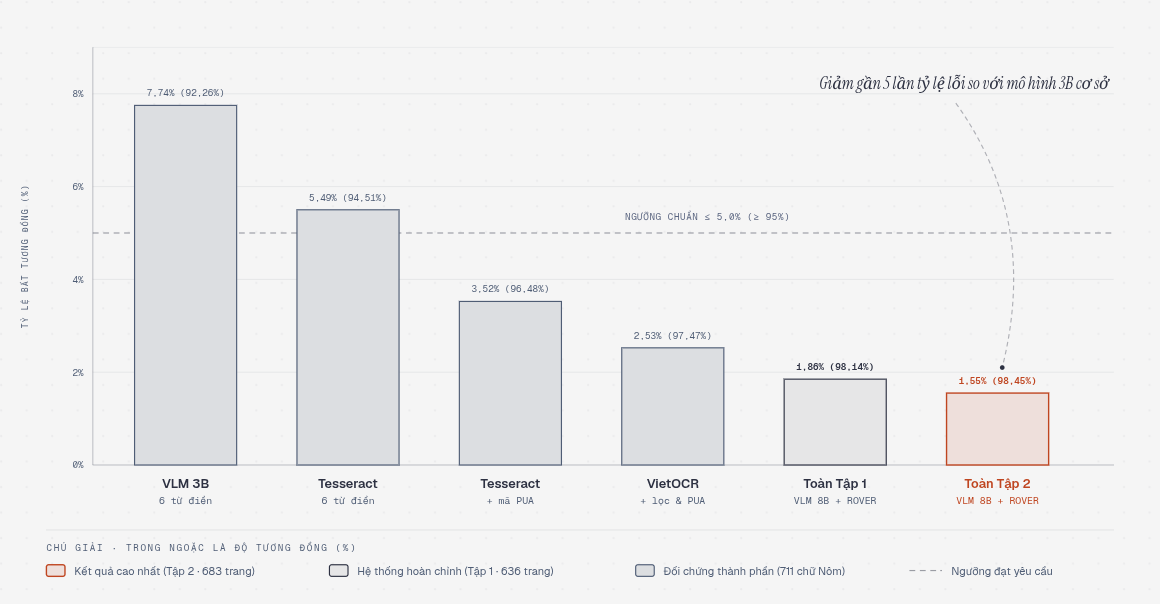
\includegraphics[width=0.95\linewidth]{images/fig3-benchmark.png}
    \caption{So sánh tỷ lệ bất tương đồng ngữ âm ($100\% - \text{Độ tương đồng}$) qua các cấu hình nhận dạng và chuẩn hóa}
    \label{fig:benchmark}
\end{figure}

\subsection{Phân tích định tính và phân rã phần dư sai khác}

Để minh họa rõ cách cơ chế ROVER liên ngôn ngữ xử lý các lỗi dấu vi mô trên dữ liệu thực tế, có thể xét một đoạn câu mang mật độ cao từ cổ và phụ âm dễ nhầm lẫn. Ở lượt đọc chính $48\text{ px}$, mô hình thị giác trả về chuỗi \textit{``Vì \textbf{chúng}, \textbf{dàng} ấy \textbf{Dấng}\ldots''}, mắc ba lỗi quen thuộc gồm nhầm \textit{ư} thành \textit{u} (tạo thành từ hiện đại \textit{chúng} vốn đúng chính tả tiếng Việt nên bộ soát lỗi đơn ngữ không phát hiện được) cùng hai lỗi mất nét ngang chữ \textit{đ} ở \textit{dàng} và \textit{Dấng}. Trong khi đó, bản đọc phụ lại nhận đúng ba từ trên nhưng đọc nhầm dấu mũ ở từ \textit{ấy}, cho ra chuỗi \textit{``Vì \textbf{chưng}, \textbf{đàng} \textbf{áy} \textbf{Đấng}\ldots''}. Khi đối chiếu với tập khóa ngữ âm trích xuất từ trang Hán Nôm đối ứng vốn có mặt các tự hình \nom{蒸} (\textit{chưng}), \nom{塘} (\textit{đàng}), \nom{等} (\textit{đấng}) và \nom{意} (\textit{ấy}), thuật toán ghi nhận khóa \code{chung}, \code{dang}, \code{dâng} không khớp tự hình nào trong vùng trang còn \code{chưng}, \code{đang}, \code{đâng} đều có đối ứng trực tiếp, nên chọn thay thế thành \textit{chưng}, \textit{đàng} và \textit{Đấng}. Ngược lại, tại vị trí \textit{ấy / áy}, khóa \code{ây} của bản chính đã khớp với chữ \nom{意} nên hệ thống giữ nguyên \textit{ấy}, tránh để sai sót từ bản phụ lan ngược vào kết quả cuối. Qua đó, câu hợp nhất đạt dạng đúng \textit{``Vì chưng, đàng ấy Đấng\ldots''} mà không một luồng đơn lẻ nào tự tạo ra được.

Bên cạnh các trường hợp được xử lý tốt, việc phân tích $2.479$ phần tử bất tương đồng còn lại trên tổng số $145.787$ tự hình tính điểm (tương ứng $1{,}86\%$ ở Tập 1 và $1{,}55\%$ ở Tập 2) cho thấy phần dư sai khác không xuất phát từ lỗi trượt ranh giới câu mà tập trung vào bốn nguyên nhân mang tính đặc thù của tư liệu lịch sử. Khoảng $45\%$ số lỗi còn lại đến từ sự thoái hóa vật lý cục bộ của bản khắc và mực in, chẳng hạn vết mọt giấy, chấm mực loang hoặc nét khắc bị gãy riêng lẻ trên từng chữ đơn khiến mô hình Hán Nôm đọc sang một chữ Hán khác bộ thủ mà không tạo thành quy luật lặp lại đủ đều để đưa vào bảng hiệu chỉnh tất định. Khoảng $25\%$ số lỗi bắt nguồn từ những biến thể dịch thuật vi mô ngay trong văn bản dịch âm 1--1, khi dịch giả đầu thế kỷ XX thỉnh thoảng thêm một hư từ tiếng Việt để câu văn tự nhiên hơn hoặc gom hai chữ Hán đẳng lập thành một từ đơn Quốc ngữ. Khoảng $25\%$ tiếp theo liên quan đến biến âm lịch sử và cách đọc địa phương thế kỷ XIX--XX xuất hiện rải rác chưa có trong bảy bộ từ điển chuẩn hóa, cùng một số rất ít tự hình lạ chưa có mục từ (trên toàn bộ $146.277$ chữ chỉ còn ba tự hình chưa có trong kho từ điển là \nom{䦕}, \ids{蔶} ở Tập 1 và \nom{𨢄} ở Tập 2). Phần nhỏ còn lại (khoảng $5\%$ tính chung các trường hợp ngoại lệ về mã hóa và ký tự hiếm) bao gồm tự hình Nôm ngoài chuẩn Unicode \nom{〓} (\ids{⿱}\nom{𥫗頓}, âm \textit{lớn}) được giữ nguyên trạng thái đánh dấu đỏ và truy vết tọa độ riêng nhằm đảm bảo tính trung thực về mặt văn bản học.

\section{Kết Luận và Hướng Phát Triển}

Báo cáo đã trình bày quy trình phương pháp luận và các thuật toán phục vụ bài toán xây dựng ngữ liệu song song mức câu giữa Hán Nôm và Quốc ngữ từ tư liệu in khắc đầu thế kỷ XX. Triển khai thực nghiệm trên hai tập của bộ \textit{Sách Dạy Đấng Làm Người Sửa Mình} ($1.319$ trang hiệu lực, $636$ đơn vị ánh xạ chính văn, $5.096$ cặp câu 1--1 với $146.277$ tự hình Hán Nôm) mang lại ba đúc kết đáng chú ý cho các bài toán số hóa văn bản cổ tương tự.

Trước hết, chất lượng dóng hàng ở giai đoạn sau phụ thuộc rất lớn vào khâu chuẩn hóa vật lý và không gian mã tự hình ở đầu vào; việc phát hiện sớm các lỗi quét đúp, xoay ngược $180^\circ$, hoán vị tay sách cùng bước quy đổi $24/25$ mã PUA sang chuẩn Unicode và khử $19$ lỗi nhầm nét có hệ thống giúp loại bỏ những nguồn nhiễu gốc mà các thuật toán so khớp chuỗi đơn thuần khó tự xử lý. Thứ hai, khi nhận dạng văn bản Quốc ngữ cổ, việc dùng chính văn bản Hán Nôm đối ứng làm tập ràng buộc ngữ âm cho bước hợp nhất ROVER giữa các giả thuyết VLM và OCR truyền thống cho thấy hiệu quả rõ rệt trong việc sửa lỗi dấu phụ và nét chữ \textit{d/đ} mà vẫn giữ lại lớp chính tả lịch sử thay vì hiện đại hóa văn bản. Thứ ba, kiến trúc quy hoạch động phân cấp hai tầng với bước chiếu ranh giới câu từ Quốc ngữ sang dòng Hán Nôm liên tục ở cấp độ cụm trang đã giúp hạn chế tình trạng trượt lệch tích lũy trên văn bản thiếu dấu câu chuẩn, duy trì tỷ lệ hàng không so sánh ở mức $0{,}00\%$ và đưa độ tương đồng chính thức đạt $98{,}14\%$ trên Tập 1 cùng $98{,}45\%$ trên Tập 2.

Trong thời gian tới, quy trình này có thể tiếp tục được mở rộng theo hai hướng chính. Ở vế Hán Nôm, cơ chế đối chứng ngữ âm có thể được phát triển theo chiều ngược lại, kết hợp khoảng cách cây cấu trúc biểu ý (IDS tree-edit distance) với âm đọc của vế Quốc ngữ nhằm gợi ý xếp hạng tự động cho các tự hình bị mờ nét cục bộ. Song song đó, việc xây dựng mô hình ngôn ngữ âm tiết chuyên biệt cho tiếng Việt thế kỷ XVII--XX sẽ giúp cải thiện thêm độ mượt cú pháp và độ chính xác của bước khôi phục phiên âm trên những trang sách bị thất lạc hoặc hư hại nặng.

\section{Bảng Phân Công Nhiệm Vụ}

Bảng~\ref{tab:contribution} tóm tắt phạm vi công việc chuyên môn, thực nghiệm và biên soạn báo cáo của hai thành viên trong quá trình thực hiện đồ án xây dựng ngữ liệu song song Hán Nôm -- Quốc ngữ.

\begin{table}[H]
    \centering
    \footnotesize
    \renewcommand{\arraystretch}{1.25}
    \begin{tabularx}{\textwidth}{l p{0.27\textwidth} X c}
        \toprule
        \textbf{Họ và tên} & \textbf{MSSV \& Email} & \textbf{Nội dung chuyên môn đảm nhiệm} & \textbf{Đóng góp} \\
        \midrule
        Nguyễn Phúc Khang & \texttt{24120068} \newline \scriptsize\texttt{24120068@student.hcmus.edu.vn}
            & Khảo sát cấu trúc vật lý ấn bản, thiết kế mô hình phân đoạn câu theo ngữ cảnh và kiến trúc quy hoạch động phân cấp hai tầng; hợp nhất kho tri thức từ điển đa nguồn cùng quan hệ dị thể; thực hiện khảo sát đối chứng các họ mô hình nhận dạng (Tesseract, VietOCR, Qwen2.5-VL-3B); thiết kế hệ thống sơ đồ, kiểm định quy cách gói nộp và biên soạn báo cáo.
            & 100\% \\
        \midrule
        Võ Quang Phúc & \texttt{24120414} \newline \scriptsize\texttt{24120414@student.hcmus.edu.vn}
            & Thiết kế luồng nhận dạng Quốc ngữ đa độ phân giải (Qwen3-VL-8B trên dòng nội suy Lanczos $48\text{ px}$ và $96\text{ px}$) cùng thuật toán hợp nhất ROVER có ràng buộc ngữ âm liên ngôn ngữ; giải mã $25$ mã tự hình PUA theo Unihan -- IDS, tổng hợp $19$ quy luật hiệu chỉnh tự hình nhầm nét và lớp âm đọc Nôm Công giáo; xử lý các dị thường bản quét (xoay ngược $180^\circ$, hoán vị tay sách), triển khai dự đoán In-Book EBMT và hoàn tất kiểm định đồng bộ 4 chiều trên cả Tập 1 và Tập 2.
            & 100\% \\
        \bottomrule
    \end{tabularx}
    \caption{Bảng phân công nhiệm vụ của các thành viên trong nhóm}
    \label{tab:contribution}
\end{table}


\newpage
\section*{Phụ Lục: Minh Họa Kiểm Chứng Định Dạng và Thực Nghiệm Trực Quan}
\addcontentsline{toc}{section}{Phụ lục: Minh họa kiểm chứng định dạng và thực nghiệm trực quan}

Phần phụ lục bổ sung các bằng chứng trực quan nhằm xác minh tính hợp lệ của dữ liệu đầu ra theo quy định hiện hành. Trước hết, các hình từ Hình~\ref{fig:ppocr_ch} đến Hình~\ref{fig:csv_preview} kiểm chứng trực tiếp định dạng hộp tọa độ bốn điểm chuẩn PPOCRLabel trên trang Hán Nôm và trang Quốc ngữ, khả năng mở tệp bảng tính \texttt{.xlsx} với đầy đủ màu chữ ngữ nghĩa không lỗi font, cũng như tính nhất quán năm cột của tệp \texttt{.csv}. Tiếp theo, Hình~\ref{fig:line_boxes} và Hình~\ref{fig:parallel_align} minh họa kết quả tách dòng trên giấy ố vàng và kết quả chiếu ranh giới câu song ngữ giữa hai hệ chữ viết đọc ngược chiều.

\subsection*{A. Kiểm chứng chuẩn định dạng PPOCRLabel, trang tính \texttt{.xlsx} và \texttt{.csv}}

\begin{figure}[H]
    \centering
    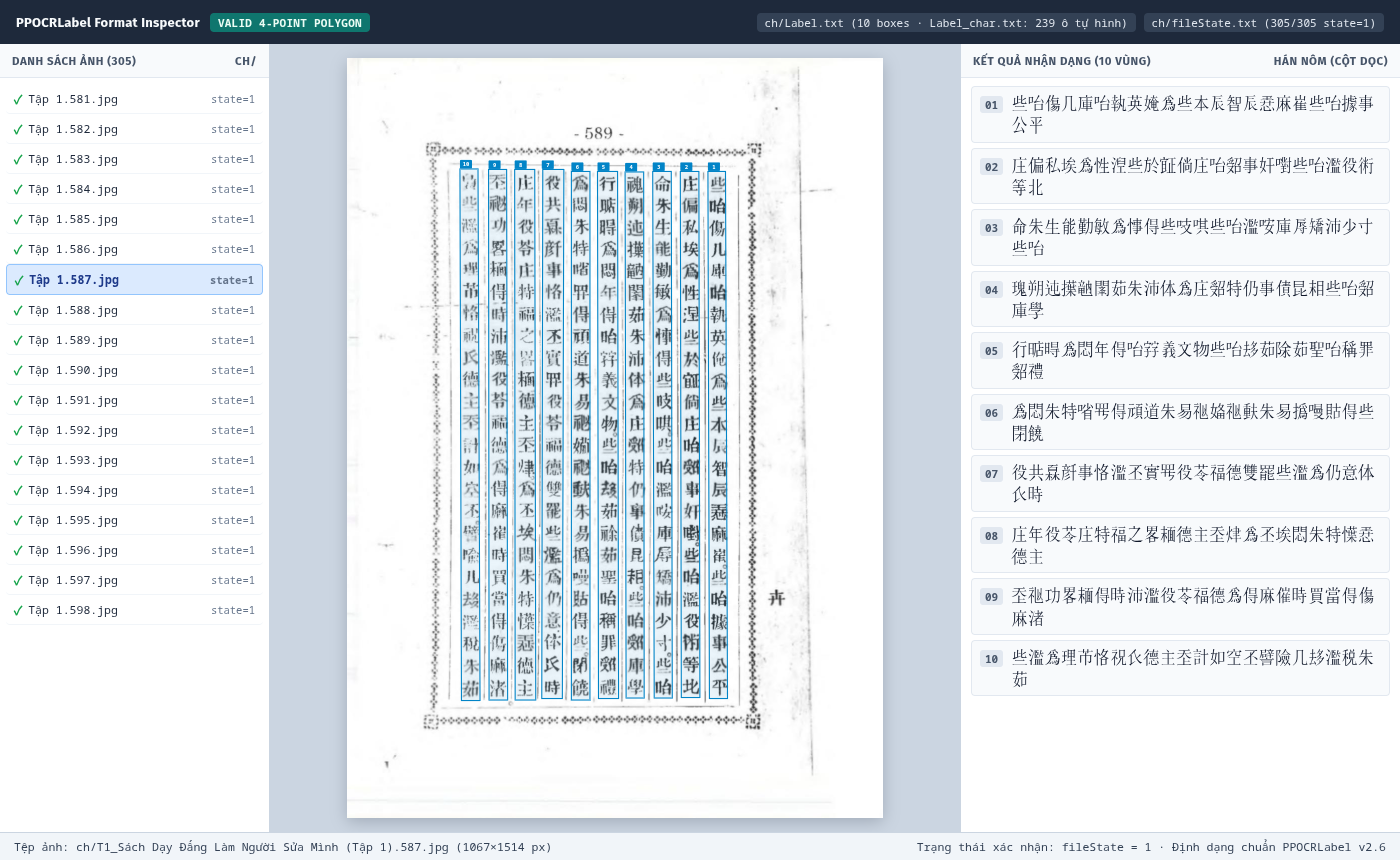
\includegraphics[width=\linewidth]{images/appendix_ppocr_ch.png}
    \caption{Kiểm chứng trực quan định dạng PPOCRLabel trên trang Hán Nôm mẫu (Tập 1, trang $587$): toàn bộ $10$ cột chữ dọc khớp khung đa giác $4$ điểm, trạng thái xác nhận hợp lệ trên $305/305$ trang cùng $239$ khung tự hình đơn}
    \label{fig:ppocr_ch}
\end{figure}

\begin{figure}[H]
    \centering
    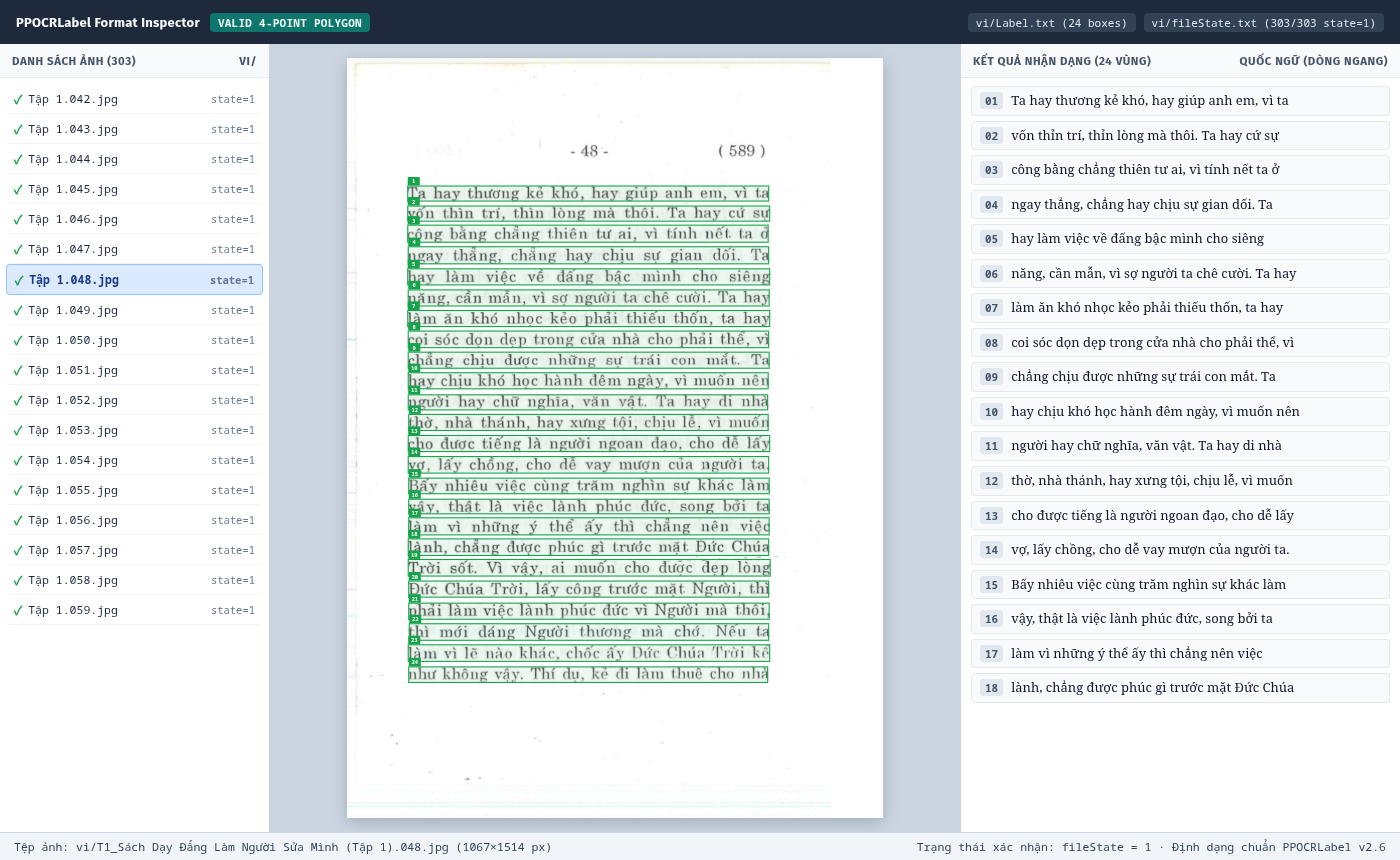
\includegraphics[width=\linewidth]{images/appendix_ppocr_vi.png}
    \caption{Kiểm chứng trực quan định dạng PPOCRLabel trên trang Quốc ngữ mẫu (Tập 1, trang $048$): toàn bộ $24$ dòng thân trang khớp khung đa giác $4$ điểm, dòng tiêu đề số trang đã được tách bỏ, trạng thái xác nhận hợp lệ trên $303/303$ trang}
    \label{fig:ppocr_vi}
\end{figure}

\begin{figure}[H]
    \centering
    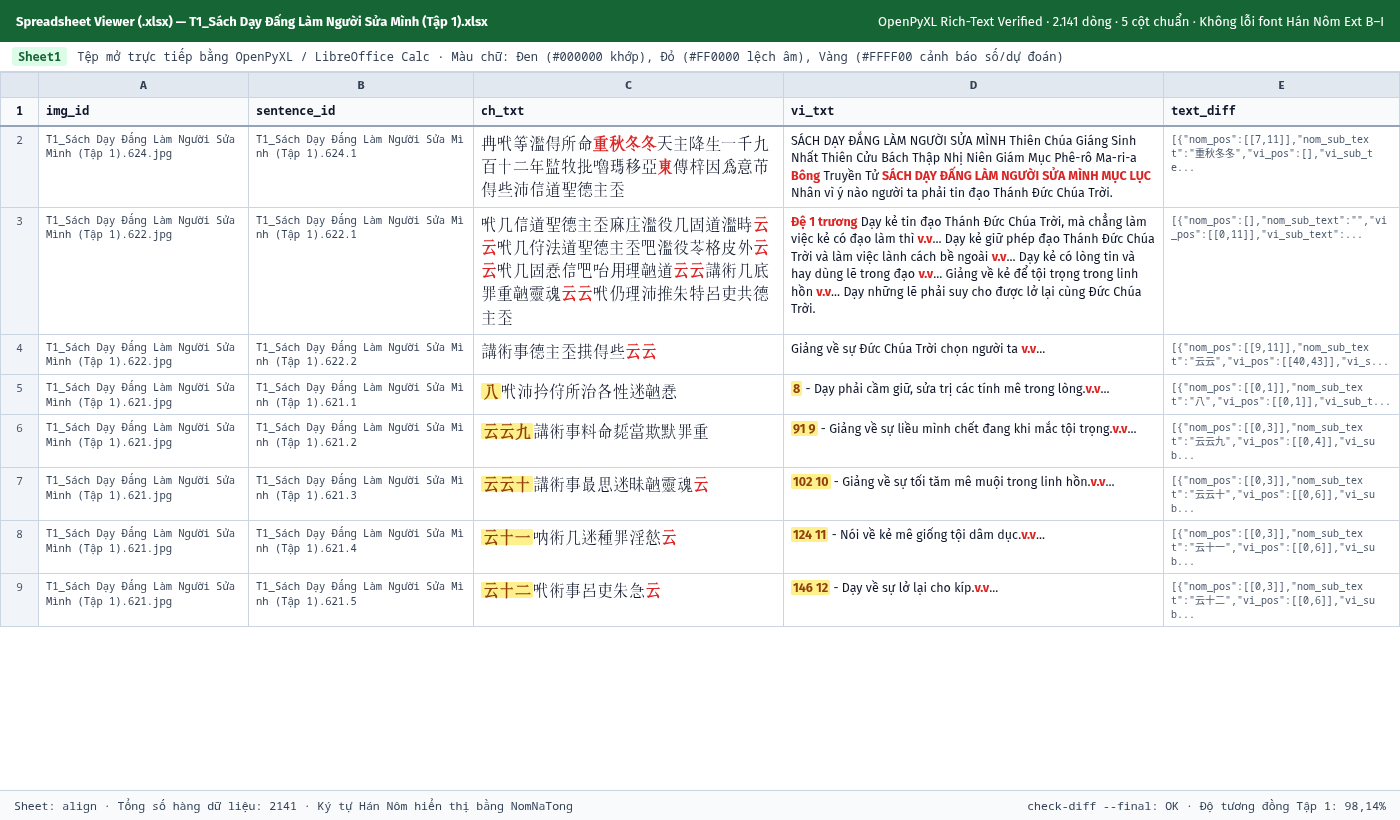
\includegraphics[width=\linewidth]{images/appendix_xlsx_preview.png}
    \caption{Kiểm chứng trang tính \texttt{.xlsx} của Tập 1 (hiển thị dữ liệu rich-text đọc trực tiếp từ tệp nộp): các tự hình Hán Nôm mở rộng hiển thị rõ nét không lỗi font và giữ đúng ba màu ngữ nghĩa (đen: khớp âm, đỏ: bất tương đồng, vàng: cảnh báo số học)}
    \label{fig:xlsx_preview}
\end{figure}

\begin{figure}[H]
    \centering
    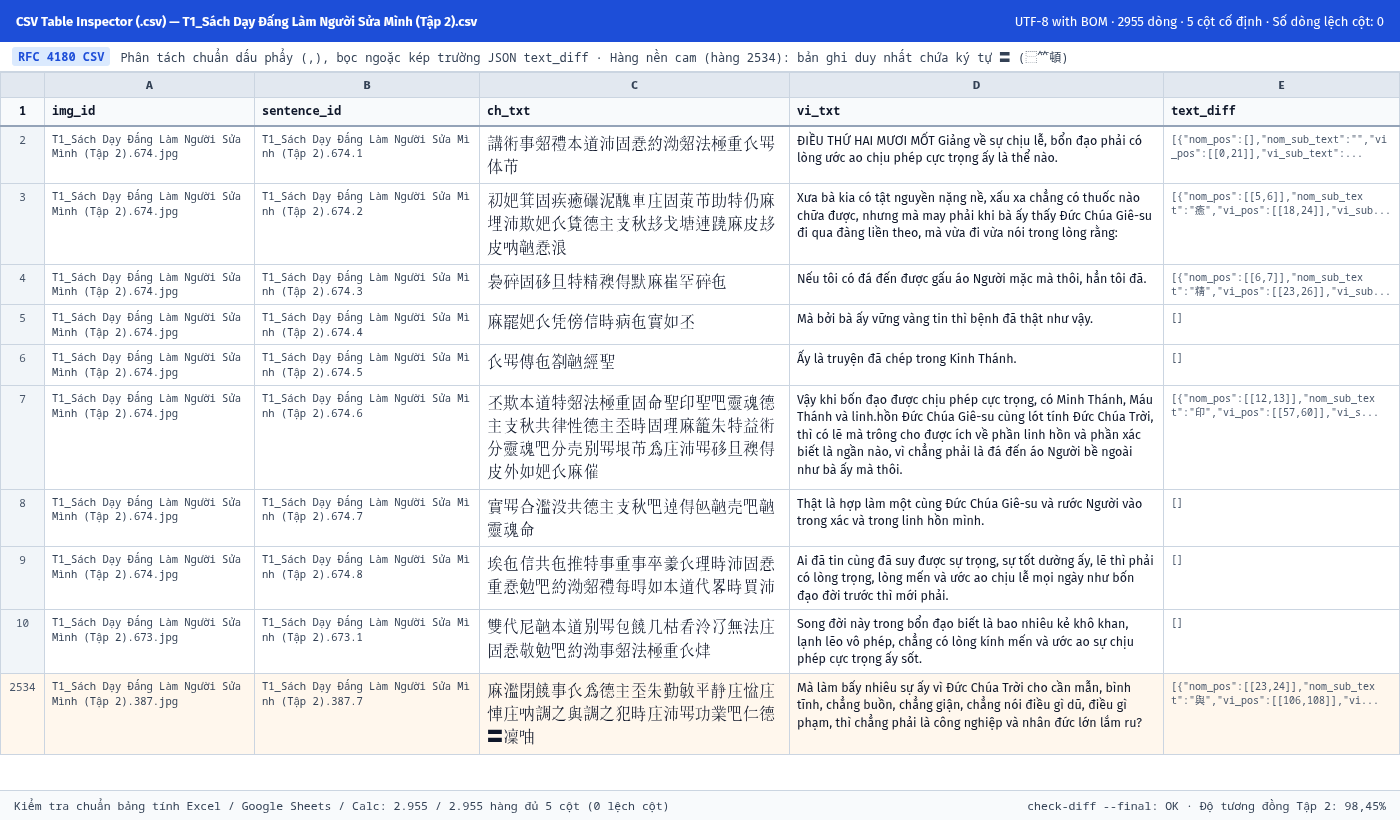
\includegraphics[width=\linewidth]{images/appendix_csv_preview.png}
    \caption{Kiểm chứng trang tính \texttt{.csv} của Tập 2 (mã hóa UTF-8 có BOM, $2.955$ dòng đủ đúng $5$ cột, $0$ dòng lệch cột): hàng nổi bật cuối cùng minh họa bản ghi duy nhất trên hai tập chứa ký tự đại diện ngoài chuẩn Unicode \nom{〓} (\ids{⿱}\nom{𥫗頓}, âm \textit{lớn})}
    \label{fig:csv_preview}
\end{figure}

\subsection*{B. Minh họa thực nghiệm tách dòng và chiếu ranh giới câu song ngữ}

\begin{figure}[H]
    \centering
    \begin{subfigure}[t]{0.48\linewidth}
        \centering
        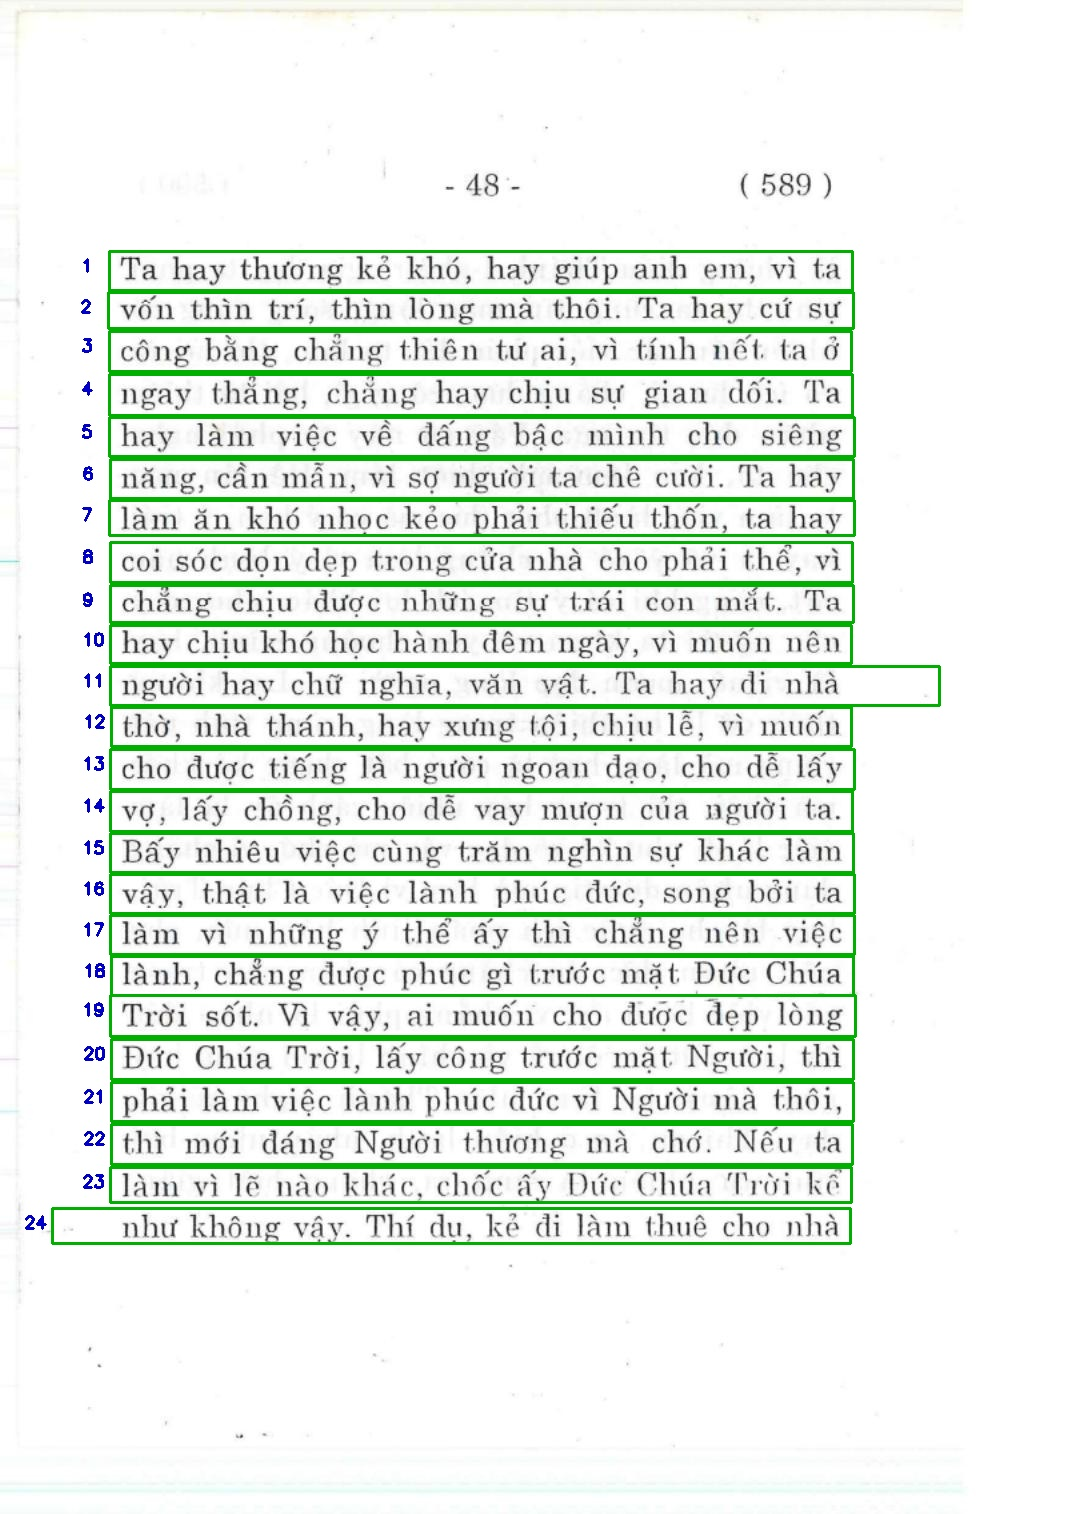
\includegraphics[width=\linewidth, height=0.38\textheight, keepaspectratio]{images/preview_048_boxes.jpg}
        \caption{Trang Quốc ngữ nền sáng tiêu chuẩn (trang in $-48-$)}
    \end{subfigure}\hfill
    \begin{subfigure}[t]{0.48\linewidth}
        \centering
        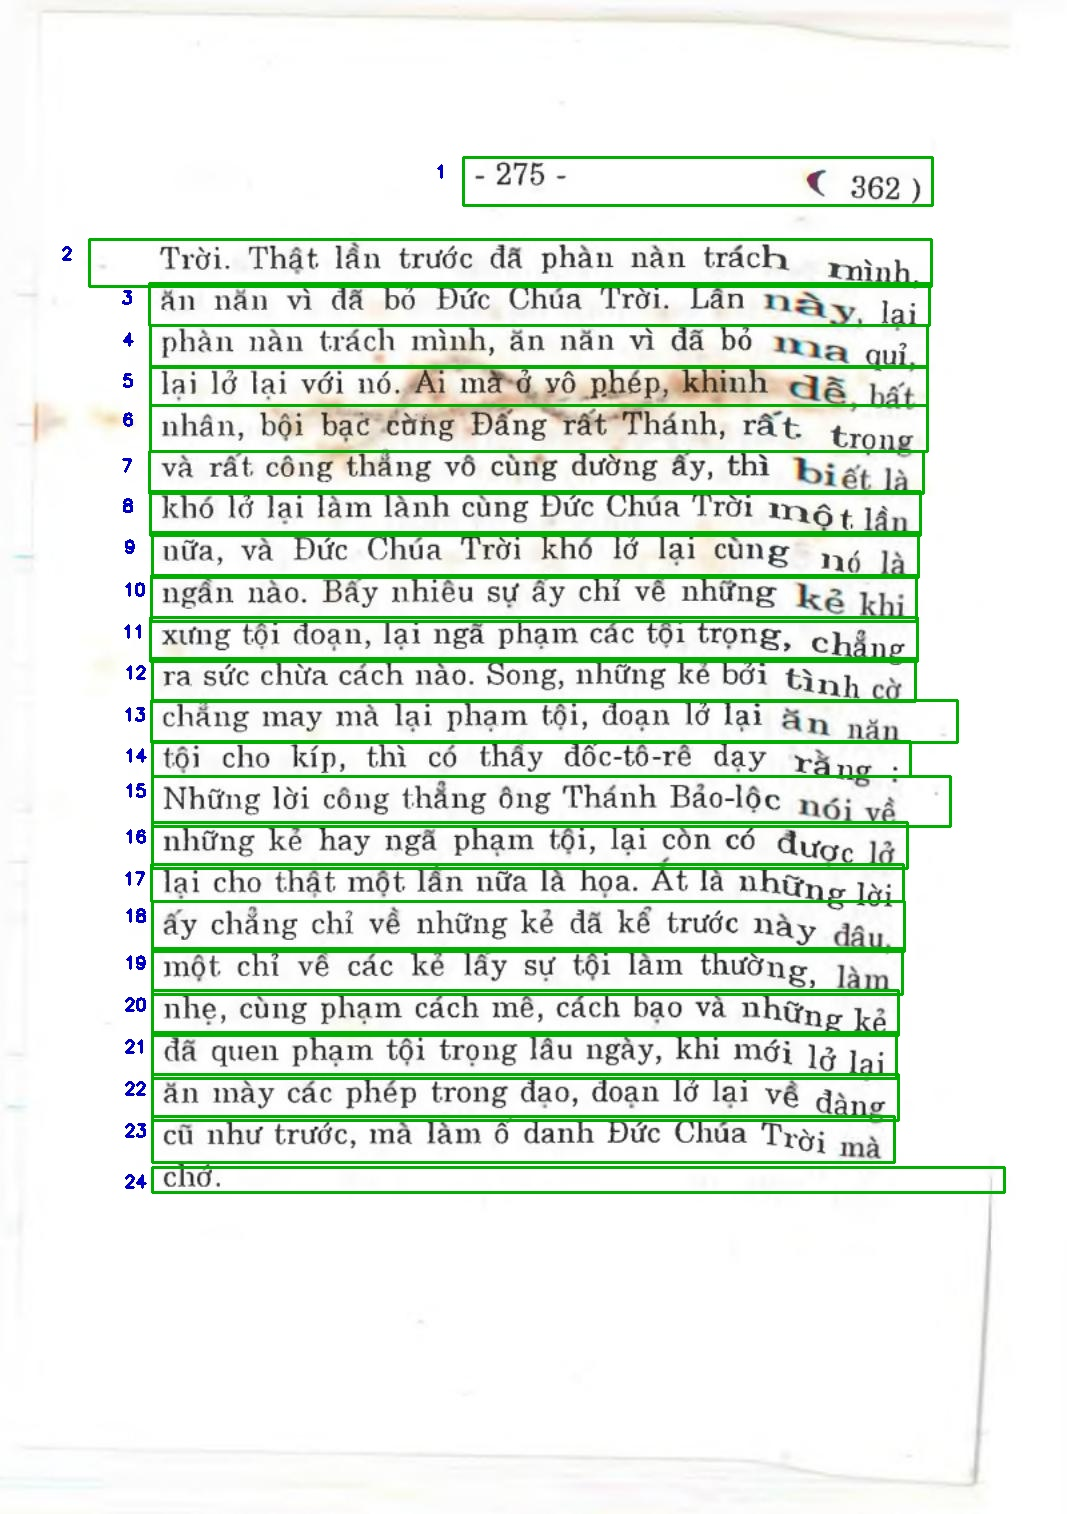
\includegraphics[width=\linewidth, height=0.38\textheight, keepaspectratio]{images/preview_275_boxes.jpg}
        \caption{Trang Quốc ngữ ố vàng nặng (trang in $-275-$)}
    \end{subfigure}
    \caption{Minh họa định vị khung dòng bốn điểm trên ấn bản Quốc ngữ đầu thế kỷ XX cho thấy ranh giới tách biệt giữa dòng tiêu đề số trang và vùng thân trang}
    \label{fig:line_boxes}
\end{figure}

\begin{figure}[H]
    \centering
    \begin{subfigure}[t]{0.48\linewidth}
        \centering
        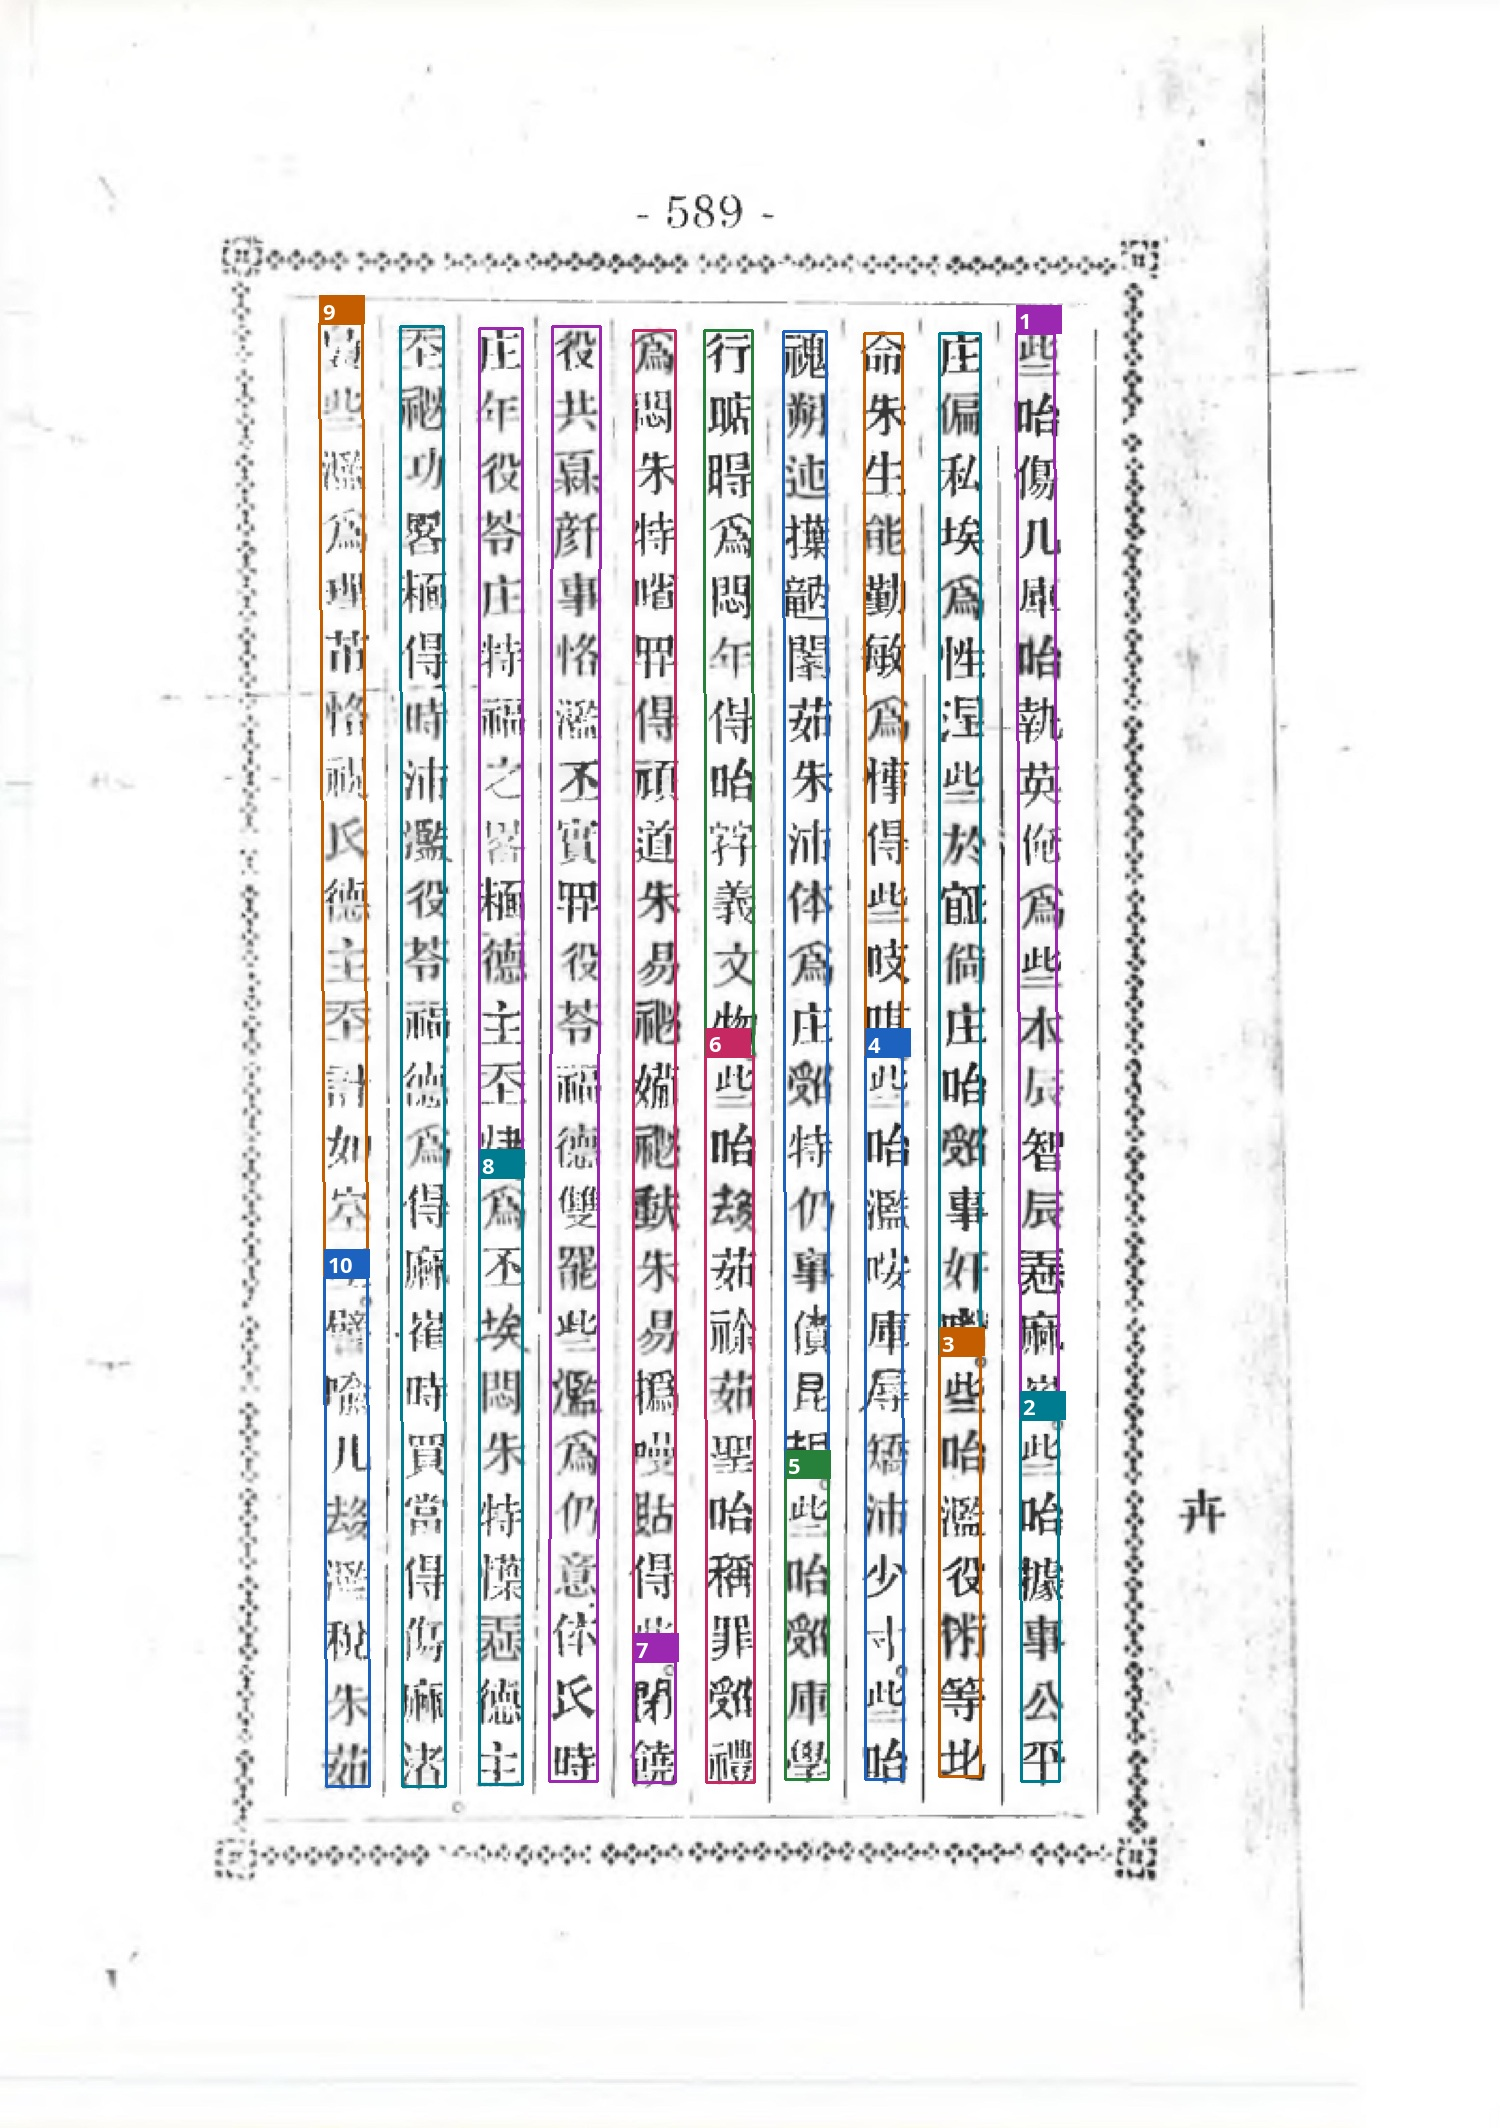
\includegraphics[width=\linewidth, height=0.38\textheight, keepaspectratio]{images/ch_annotated.jpg}
        \caption{Vế Hán Nôm đọc dọc phải sang trái (trang in $-589-$)}
    \end{subfigure}\hfill
    \begin{subfigure}[t]{0.48\linewidth}
        \centering
        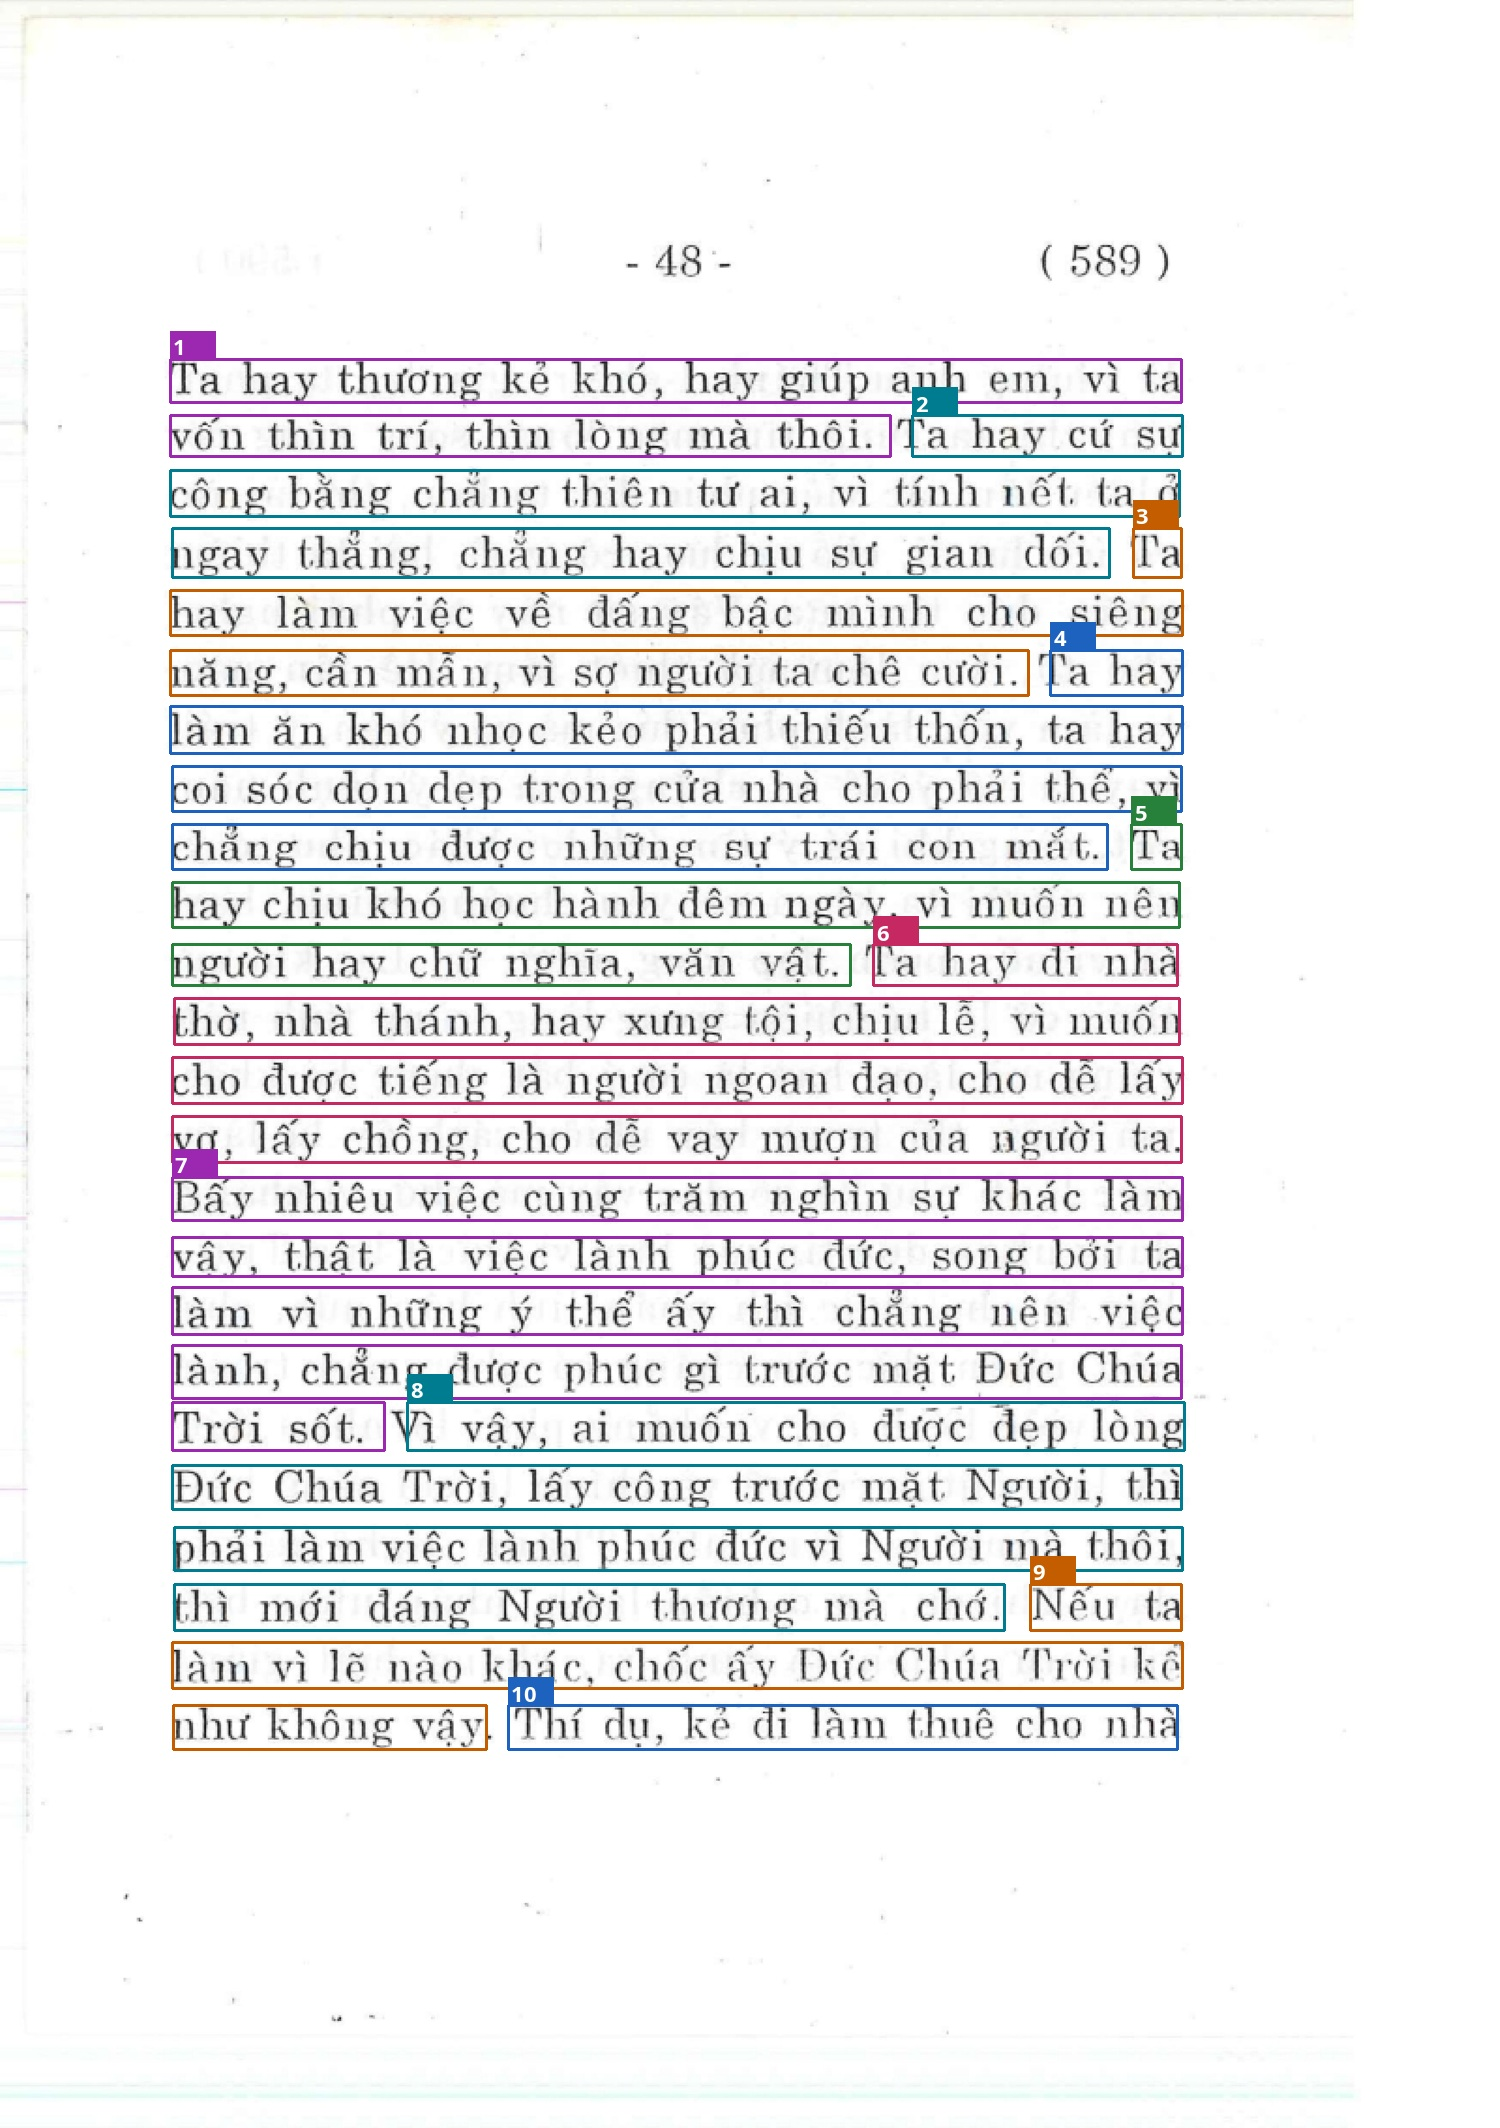
\includegraphics[width=\linewidth, height=0.38\textheight, keepaspectratio]{images/vi_annotated.jpg}
        \caption{Vế Quốc ngữ đọc ngang trái sang phải (trang in $-48-$)}
    \end{subfigure}
    \caption{Minh họa kết quả chiếu ranh giới câu bằng quy hoạch động hai tầng trên cặp trang đối ứng thực tế với $10$ câu song ngữ được khoanh vùng đồng bộ mã màu giữa hai hệ chữ viết}
    \label{fig:parallel_align}
\end{figure}


\newpage
\addcontentsline{toc}{section}{Tài liệu tham khảo}
\bibliographystyle{IEEEtran}
\bibliography{ref}

\end{document}
